%% abtex2-modelo-trabalho-academico.tex, v-1.9.6 laurocesar
%% Copyright 2012-2016 by abnTeX2 group at http://www.abntex.net.br/ 
%%
%% This work may be distributed and/or modified under the
%% conditions of the LaTeX Project Public License, either version 1.3
%% of this license or (at your option) any later version.
%% The latest version of this license is in
%%   http://www.latex-project.org/lppl.txt
%% and version 1.3 or later is part of all distributions of LaTeX
%% version 2005/12/01 or later.
%%
%% This work has the LPPL maintenance status `maintained'.
%% 
%% The Current Maintainer of this work is the abnTeX2 team, led
%% by Lauro César Araujo. Further information are available on 
%% http://www.abntex.net.br/
%%
%% This work consists of the files abntex2-modelo-trabalho-academico.tex,
%% abntex2-modelo-include-comandos and abntex2-modelo-references.bib
%%

% ------------------------------------------------------------------------
% ------------------------------------------------------------------------
% abnTeX2: Modelo de Trabalho Academico (tese de doutorado, dissertacao de
% mestrado e trabalhos monograficos em geral) em conformidade com 
% ABNT NBR 14724:2011: Informacao e documentacao - Trabalhos academicos -
% Apresentacao
% ------------------------------------------------------------------------
% ------------------------------------------------------------------------

\documentclass[
	% -- opções da classe memoir --
	12pt,				% tamanho da fonte
	openright,			% capítulos começam em pág ímpar (insere página vazia caso preciso)
	twoside,			% para impressão em recto e verso. Oposto a oneside
	a4paper,			% tamanho do papel. 
	% -- opções da classe abntex2 --
	%chapter=TITLE,		% títulos de capítulos convertidos em letras maiúsculas
	%section=TITLE,		% títulos de seções convertidos em letras maiúsculas
	%subsection=TITLE,	% títulos de subseções convertidos em letras maiúsculas
	%subsubsection=TITLE,% títulos de subsubseções convertidos em letras maiúsculas
	% -- opções do pacote babel --
	english,			% idioma adicional para hifenização
	french,				% idioma adicional para hifenização
	spanish,			% idioma adicional para hifenização
	brazil				% o último idioma é o principal do documento
	]{abntex2}

% ---
% Pacotes básicos 
% ---
\usepackage{lmodern}			% Usa a fonte Latin Modern			
\usepackage[T1]{fontenc}		% Selecao de codigos de fonte.
\usepackage[utf8]{inputenc}		% Codificacao do documento (conversão automática dos acentos)
\usepackage{lastpage}			% Usado pela Ficha catalográfica
\usepackage{indentfirst}		% Indenta o primeiro parágrafo de cada seção.
\usepackage{color}				% Controle das cores
\usepackage{graphicx}			% Inclusão de gráficos
\usepackage{microtype} 			% para melhorias de justificação
% ---
\usepackage[utf8]{inputenc}
\usepackage{listings}
\usepackage{xcolor}
\usepackage[compact]{titlesec}
\titlespacing{\section}{0pt}{*0}{*0}
\titlespacing{\subsection}{0pt}{*0}{*0}
\titlespacing{\subsubsection}{0pt}{*0}{*0}

		
% ---
% Pacotes adicionais, usados apenas no âmbito do Modelo Canônico do abnteX2
% ---
\usepackage{lipsum}				% para geração de dummy text
% ---

% ---
% Pacotes de citações
% ---
\usepackage[brazilian,hyperpageref]{backref}	 % Paginas com as citações na bibl
\usepackage[alf]{abntex2cite}	% Citações padrão ABNT
\usepackage{cite}
\usepackage{hyperref}
\usepackage{cleveref}
\setcounter{tocdepth}{5}

% --- 
% CONFIGURAÇÕES DE PACOTES
% --- 

% ---
% Configurações do pacote backref
% Usado sem a opção hyperpageref de backref
\renewcommand{\backrefpagesname}{Citado na(s) página(s):~}
% Texto padrão antes do número das páginas
\renewcommand{\backref}{}
% Define os textos da citação
\renewcommand*{\backrefalt}[4]{
	\ifcase #1 %
		Nenhuma citação no texto.%
	\or
		Citado na página #2.%
	\else
		Citado #1 vezes nas páginas #2.%
	\fi}%
% ---

% ---
% Informações de dados para CAPA e FOLHA DE ROSTO
% ---
\titulo{Aplicativo móvel para educação ambiental}
\autor{Flávio Telles Paschoal Santos}
\local{Rio das Ostras}
\data{2018}
\orientador{Carlos Basílio}
\coorientador{Flávio Machado}
\instituicao{%
  UNIVERSIDADE FEDERAL FLUMINENSE
  \par
  PÓLO UNIVERSITÁRIO DE RIO DAS OSTRAS
  \par
   \par
  INSTITUTO DE CIÊNCIA E TECNOLOGIA
  \par
 CURSO DE BACHARELADO EM CIÊNCIA DA COMPUTAÇÃO}
\tipotrabalho{Trabalho de conclusão de curso (Bacharelado)}
% O preambulo deve conter o tipo do trabalho, o objetivo, 
% o nome da instituição e a área de concentração 
\preambulo{}
% ---


% ---
% Configurações de aparência do PDF final

% alterando o aspecto da cor azul
\definecolor{blue}{RGB}{41,5,195}
% Definindo novas cores
\definecolor{verde}{rgb}{0.25,0.5,0.35}
\definecolor{jpurple}{rgb}{0.5,0,0.35}
\definecolor{dkgreen}{rgb}{0,.6,0}
\definecolor{dkblue}{rgb}{0,0,.6}
\definecolor{dkyellow}{cmyk}{0,0,.8,.3}
% Configurando layout para mostrar codigos Java
\usepackage{listings}
\lstset{
     literate=%
         {á}{{\'a}}1
         {ã}{{\~a}}1
         {â}{{\^a}}1
         {í}{{\'i}}1
         {é}{{\'e}}1
         {ê}{{\^e}}1
         {ú}{{\'u}}1
         {ó}{{\'o}}1
         {õ}{{\~o}}1
}
\lstset{
  language=Java,
  basicstyle=\ttfamily\small,
  keywordstyle=\color{jpurple}\bfseries,
  stringstyle=\color{red},
  commentstyle=\color{verde},
  morecomment=[s][\color{blue}]{/**}{*/},
  extendedchars=true,
  showspaces=false,
  showstringspaces=false,
  numbers=left,
  numberstyle=\tiny,
  breaklines=true,
  backgroundcolor=\color{cyan!10},
  breakautoindent=true,
  captionpos=b,
  xleftmargin=0pt,
  tabsize=4
}
\lstdefinelanguage{XML}{
  basicstyle=\ttfamily\footnotesize,
  morestring=[b]",
  moredelim=[s][\bfseries\color{Maroon}]{<}{\ },
  moredelim=[s][\bfseries\color{Maroon}]{</}{>},
  moredelim=[l][\bfseries\color{Maroon}]{/>},
  moredelim=[l][\bfseries\color{Maroon}]{>},
  morecomment=[s]{<?}{?>},
  morecomment=[s]{<!--}{-->},
  commentstyle=\color{DarkOliveGreen},
  stringstyle=\color{blue},
  identifierstyle=\color{black}
}
% ---

% informações do PDF
\makeatletter
\hypersetup{
     	%pagebackref=true,
		pdftitle={\@title}, 
		pdfauthor={\@author},
    	pdfsubject={\imprimirpreambulo},
	    pdfcreator={LaTeX with abnTeX2},
		pdfkeywords={abnt}{latex}{abntex}{abntex2}{trabalho acadêmico}, 
		colorlinks=true,       		% false: boxed links; true: colored links
    	linkcolor=blue,          	% color of internal links
    	citecolor=blue,        		% color of links to bibliography
    	filecolor=magenta,      		% color of file links
		urlcolor=blue,
		bookmarksdepth=4
}
\makeatother
% --- 

% --- 
% Espaçamentos entre linhas e parágrafos 
% --- 

% O tamanho do parágrafo é dado por:
\setlength{\parindent}{1.3cm}

% Controle do espaçamento entre um parágrafo e outro:
\setlength{\parskip}{0.2cm}  % tente também \onelineskip

% ---
% compila o indice
% ---
\makeindex
% ---

% ----
% Início do documento
% ----
\begin{document}

% Seleciona o idioma do documento (conforme pacotes do babel)
%\selectlanguage{english}
\selectlanguage{brazil}

% Retira espaço extra obsoleto entre as frases.
\frenchspacing 

% ----------------------------------------------------------
% ELEMENTOS PRÉ-TEXTUAIS
% ----------------------------------------------------------
% \pretextual

% ---
% Capa
% ---
\imprimircapa
% ---

% ---
% Folha de rosto
% (o * indica que haverá a ficha bibliográfica)
% ---
\imprimirfolhaderosto
% ---



% ---
% Inserir folha de aprovação
% ---

% Isto é um exemplo de Folha de aprovação, elemento obrigatório da NBR
% 14724/2011 (seção 4.2.1.3). Você pode utilizar este modelo até a aprovação
% do trabalho. Após isso, substitua todo o conteúdo deste arquivo por uma
% imagem da página assinada pela banca com o comando abaixo:
%
% \includepdf{folhadeaprovacao_final.pdf}
%
\begin{folhadeaprovacao}

  \begin{center}
    {\ABNTEXchapterfont\large\imprimirautor}

    \vspace*{\fill}\vspace*{\fill}
    \begin{center}
      \ABNTEXchapterfont\bfseries\Large\imprimirtitulo
    \end{center}
    \vspace*{\fill}
    
    \hspace{.45\textwidth}
    \begin{minipage}{.5\textwidth}
        \imprimirpreambulo
    \end{minipage}%
    \vspace*{\fill}
   \end{center}
        
   Trabalho aprovado. \imprimirlocal, 15 de dezembro de 2018:

   \assinatura{\textbf{\imprimirorientador} \\ Orientador} 
   \assinatura{\textbf{Professor} \\ Convidado 1}
   \assinatura{\textbf{Professor} \\ Convidado 2}
   %\assinatura{\textbf{Professor} \\ Convidado 3}
   %\assinatura{\textbf{Professor} \\ Convidado 4}
      
   \begin{center}
    \vspace*{0.5cm}
    {\large\imprimirlocal}
    \par
    {\large\imprimirdata}
    \vspace*{1cm}
  \end{center}
  
\end{folhadeaprovacao}
% ---

% ---
% Dedicatória
% ---
\begin{dedicatoria}
   \vspace*{\fill}
   \centering
   \noindent
   \textit{ Este trabalho é dedicado às crianças adultas que,\\
   quando pequenas, sonharam em se tornar cientistas.} \vspace*{\fill}
\end{dedicatoria}
% ---

% ---
% Agradecimentos
% ---
\begin{agradecimentos}


\end{agradecimentos}
% ---




% ---
% RESUMOS
% ---

% resumo em português
\setlength{\absparsep}{18pt} % ajusta o espaçamento dos parágrafos do resumo
\begin{resumo}

 O Brasil produz lixo em quantidades semelhantes à de países desenvolvidos, porem suas políticas e infraestrutura de descarte são equivalentes à de países pobres. A falta de infraestrutura para o recolhimento do lixo é o principal vilão quando se trata de reciclagem, somente 2\% de todo lixo produzido é reciclado.
	Segundo o IBGE em 2015, 77.1\% dos brasileiros possuem um telefone celular e 64.7\% possuem acesso à internet. Logo, o presente trabalho tem como objetivo facilitar o acesso às informações por meio do uso da tecnologia móvel para incentivar aqueles que tem acesso à infraestrutura a descartar corretamente os materiais. Os acessos às informações serão disponibilizados através de um aplicativo que será desenvolvido ao longo desse projeto para que os usuários possam ter um melhor entendimento dos problemas econômicos e sociais causados pelo lixo não reciclado de modo que esses usuários possam desenvolver uma consciência crítica sobre o descarte do lixo doméstico.


 \textbf{Palavras-chave}: Reciclagem, Tecnologia móvel.
\end{resumo}

% resumo em inglês
\begin{resumo}[Abstract]
 \begin{otherlanguage*}{english}
   Brazil produces garbage in quantities similar to those of developed countries, but its policies and disposal infrastructure are equivalent to those of poor countries. The lack of infrastructure for garbage collection is the main villain when it comes to recycling, only 2 \% of all garbage produced is recycled.
According to IBGE in 2015, 77.1 \% of Brazilians have a cell phone and 64.7 \% have access to the internet. Therefore, the present work aims to facilitate access to information through the use of mobile technology to encourage those who have access to the infrastructure to properly discard the materials. Access to information will be made available through an application that will be developed throughout this project so that users can gain a better understanding of the economic and social problems caused by non-recycled litter so that users can develop a critical awareness of the disposal of domestic waste.

   \vspace{\onelineskip}
 
   \noindent 
   \textbf{Keywords}: Recycling, Mobile Technology.
 \end{otherlanguage*}
\end{resumo}



% ---
% inserir lista de ilustrações
% ---
\pdfbookmark[0]{\listfigurename}{lof}
\listoffigures*
\cleardoublepage
% ---

% ---
% inserir lista de tabelas
% ---
\pdfbookmark[0]{\listtablename}{lot}
\listoftables*
\cleardoublepage
% ---

% ---
% inserir lista de abreviaturas e siglas
% ---
\begin{siglas}
  \item[SDK] Software Development Kit  
\end{siglas}
% ---



% ---
% inserir lista de símbolos
% ---
%\begin{simbolos}
%  \item[$ \Gamma $] Letra grega Gama
%  \item[$ \Lambda $] Lambda
%  \item[$ \zeta $] Letra grega minúscula zeta
%  \item[$ \in $] Pertence
%\end{simbolos}
% ---

% ---
% inserir o sumario
% ---


\pdfbookmark[0]{\contentsname}{toc}
\tableofcontents*
\cleardoublepage

% ---



% ----------------------------------------------------------
% ELEMENTOS TEXTUAIS
% ----------------------------------------------------------
\textual

% ----------------------------------------------------------
% Introdução (exemplo de capítulo sem numeração, mas presente no Sumário)
% ----------------------------------------------------------




% ----------------------------------------------------------
% PARTE
% ----------------------------------------------------------
\chapter{Introdução}
% ----------------------------------------------------------
\section{Motivação}
Com o aumento exponencial da população cresce também de forma exponencial o consumo de matéria prima e a quantidade de lixo produzido. Ao longo dos anos surgiram novas maneiras de reaproveitar esses materiais que antes eram descartados em lixões e aterros, como plásticos, papeis, metais e vidros. Muito desses componentes quando não descartados ou tratados de forma adequadas demoram anos e até séculos para de decompor. O acúmulo desses resíduos tem um grande impacto ambiental, destruindo ecossistemas e espécies no seu processo de decomposição. Além disso, o acúmulo desses resíduos tem um grande impacto na saúde e na economia. Os resíduos não descartados de forma correta atuam como facilitadores na disseminação de doenças, o que gera um aumento significativo dos gastos com a saúde. O impacto econômico da reciclagem vai além dos gastos convencionais com a saúde, através dessa prática é possível obter renda extra com produtos reciclados, diminuir a extração de matéria prima tornando os produtos mais baratos e incentivando empreendedores a investir neste ramo e assim gerando mais empregos diretos e indiretos. 
\section{Objetivo}
\subsection{Objetivo Geral}
O objetivo principal desse projeto é o desenvolvimento de um aplicativo mobile (software) nativo para sistemas Android, essa tecnologia permitirá usuários interessados em adquirir novos conhecimentos sobre o processo, composição e impacto dos resíduos produzidos em todo o mundo.

\subsection{Objetivos Específicos}
\begin{itemize}
	\item Este projeto também tem como objetivo entregar conteúdo dinâmico através de um painel administrativo e um serviço web, que será usado para inserir e manter o conteúdo apresentado no aplicativo.
    \item Solucionar problemas de conectividade causados pela mobilidade dos dispositivos, permitindo que o usuário acesse o conteúdo quando estiver sem acesso à internet.
        \item Solucionar problemas relacionados a dimensão de telas e garantir a retro compatibilidade com dispositivos mais antigos.
\end{itemize}
% ---

% ----------------------------------------------------------
\chapter{Trabalhos relacionados}
% ----------------------------------------------------------

Neste capítulo serão apresentados três trabalhados, dois aplicativos móveis e uma pagina da internet que possuem funcionalidades similares ao projeto atual descrito nesse documento. Funcionalidades não relevantes não serão apresentadas.

\section{Cataki}
O aplicativo atua conectando os catadores com qualquer um que tenha resíduos ou material reciclável a ser recolhido. A ideia é reconhecer o pequeno empreendedorismo ambiental desempenhado por estes profissionais e colaborar com o descarte adequado dos resíduos.

Para utilizar o aplicativo basta efetuar a transferência na Google Play\cite{googleplay} ou na App Store\cite{appstore} e começar a utiliza-lo, o Cataki permite o uso dos seus recursos de forma anônima, facilitando o acesso rápido as suas funcionalidades. É possível também, ainda de forma anônima, cadastrar um novo catador dando visibilidade aos indivíduos que tem dificuldade em manipular recursos de um aplicativo móvel, ou não possuem acesso à internet.

Na \autoref{fig:figura1} pode-se observar a funcionalidade principal do aplicativo, onde um mapa mostrando ícones nas localizações dos catadores, centros de coleta e cooperativas é exibido na tela possibilitando a interação do usuário com esses pontos. Caso um ícone seja selecionado, as informações referente a este fica disponível. A \autoref{fig:figura2} mostra a tela exibida após o ícone do catador ser selecionado, informações como o resíduo que esse catador trabalha e dados relevantes para o contato fica disponível. 
    

    \begin{figure}[htb]    
 \centering
  \begin{minipage}{0.45\textwidth}
    \centering
    \caption{Cataki - Localizar}
    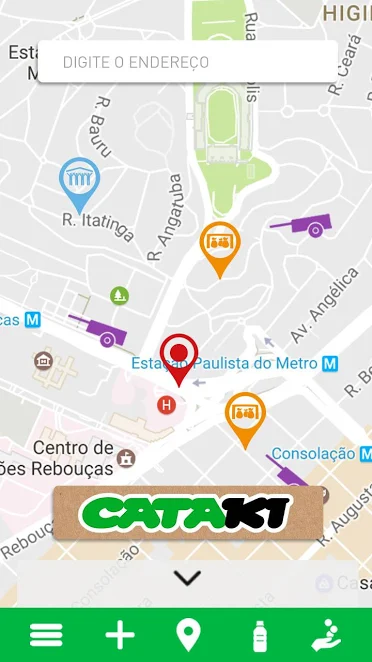
\includegraphics[scale=0.45]{media/catakimap.png}
    \legend{Fonte: Google Play}
     \label{fig:figura1}
  \end{minipage}
  \hfill
  \begin{minipage}{0.45\textwidth}
    \centering
    \caption{Cataki - Catador}
    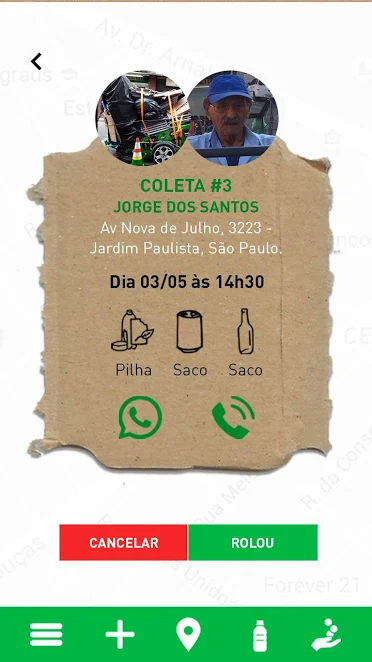
\includegraphics[scale=0.45]{media/infocatador.png}
    \legend{Fonte: Google Play}
     \label{fig:figura2}
  \end{minipage}
\end{figure}

\newpage
O Cataki também possui um banco de dados com informações genéricas sobre o descarte e sobre os materiais. A \autoref{fig:figura3} mostra os materiais disponíveis no aplicativo, quando uma material é selecionado, uma nova tela se abre mostrando os detalhes sobre o mesmo, como mostrado na \autoref{fig:figura4}. \\
     \begin{figure}[htb]    
 \centering
  \begin{minipage}{0.45\textwidth}
    \centering
    \caption{Cataki - Materiais}
    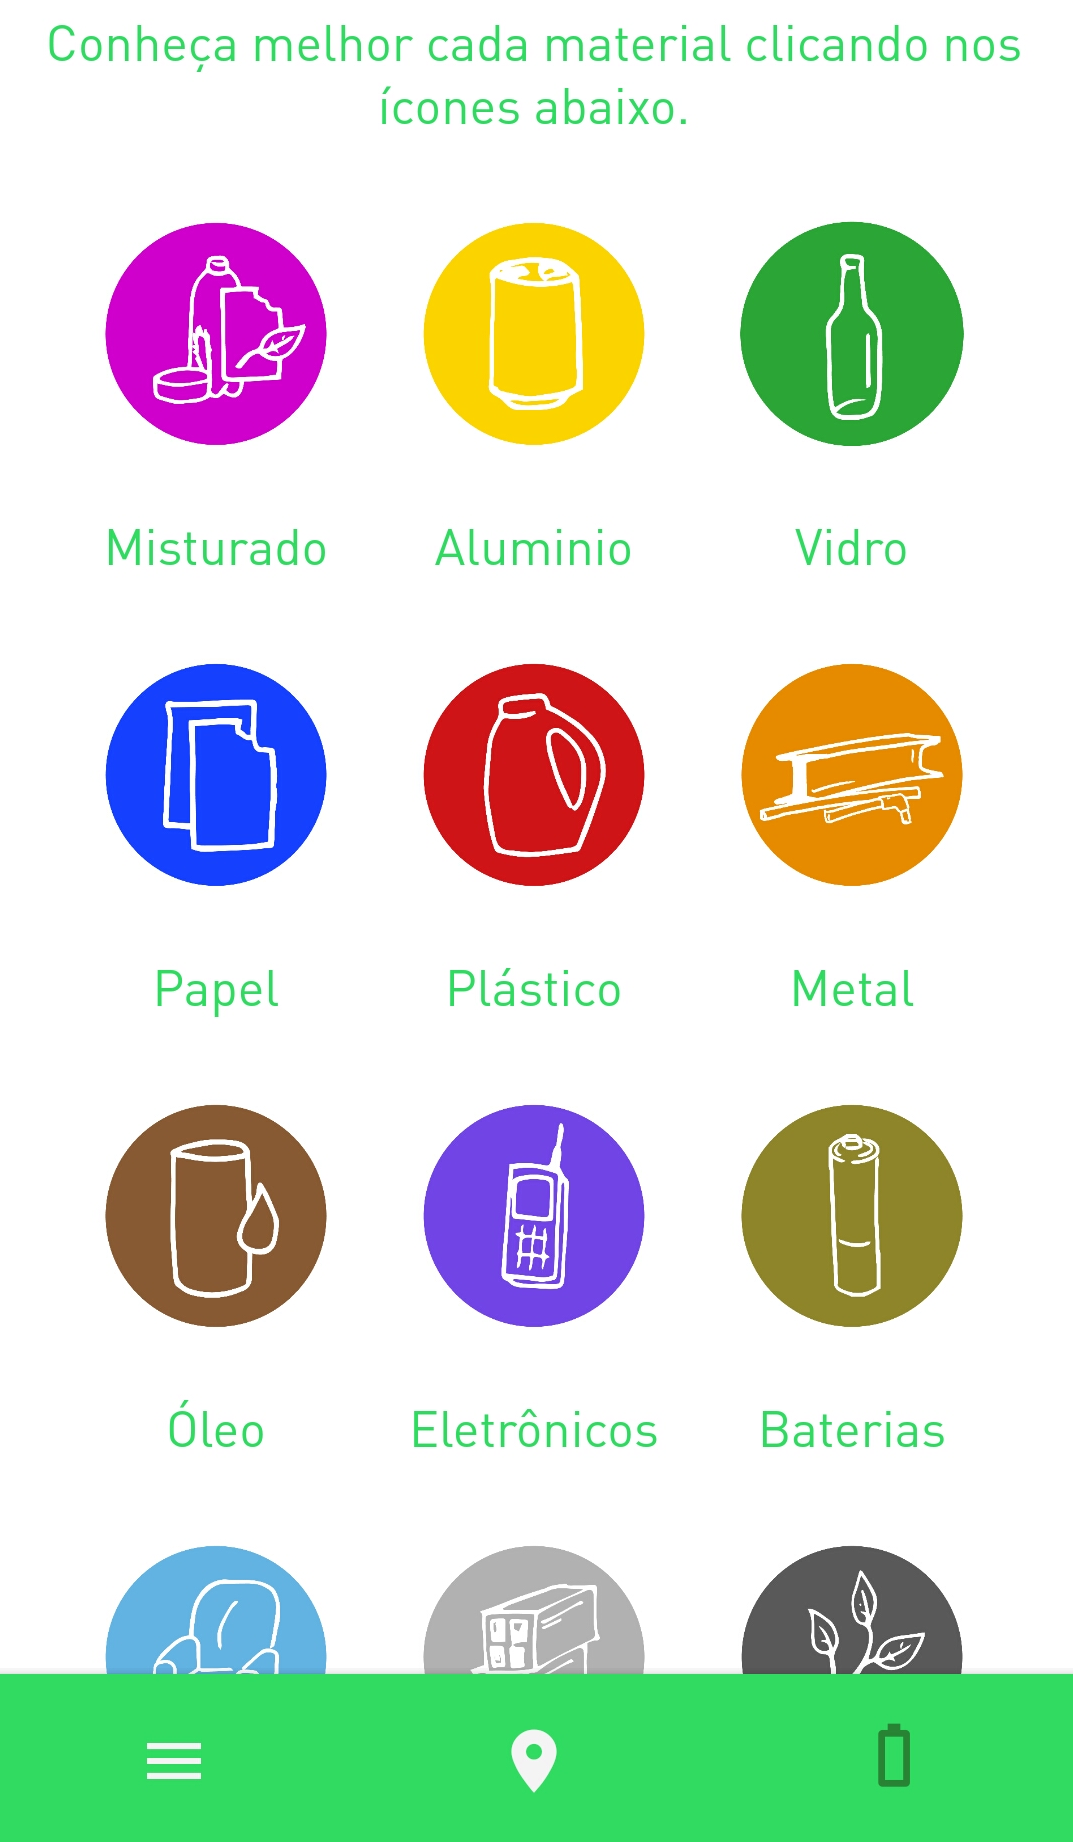
\includegraphics[scale=0.15]{media/catakimateriais.png}   
    \legend{Fonte: Google Play}
     \label{fig:figura3}
  \end{minipage}
  \hfill
  \begin{minipage}{0.45\textwidth}
    \centering
    \caption{Cataki - Detalhes}
    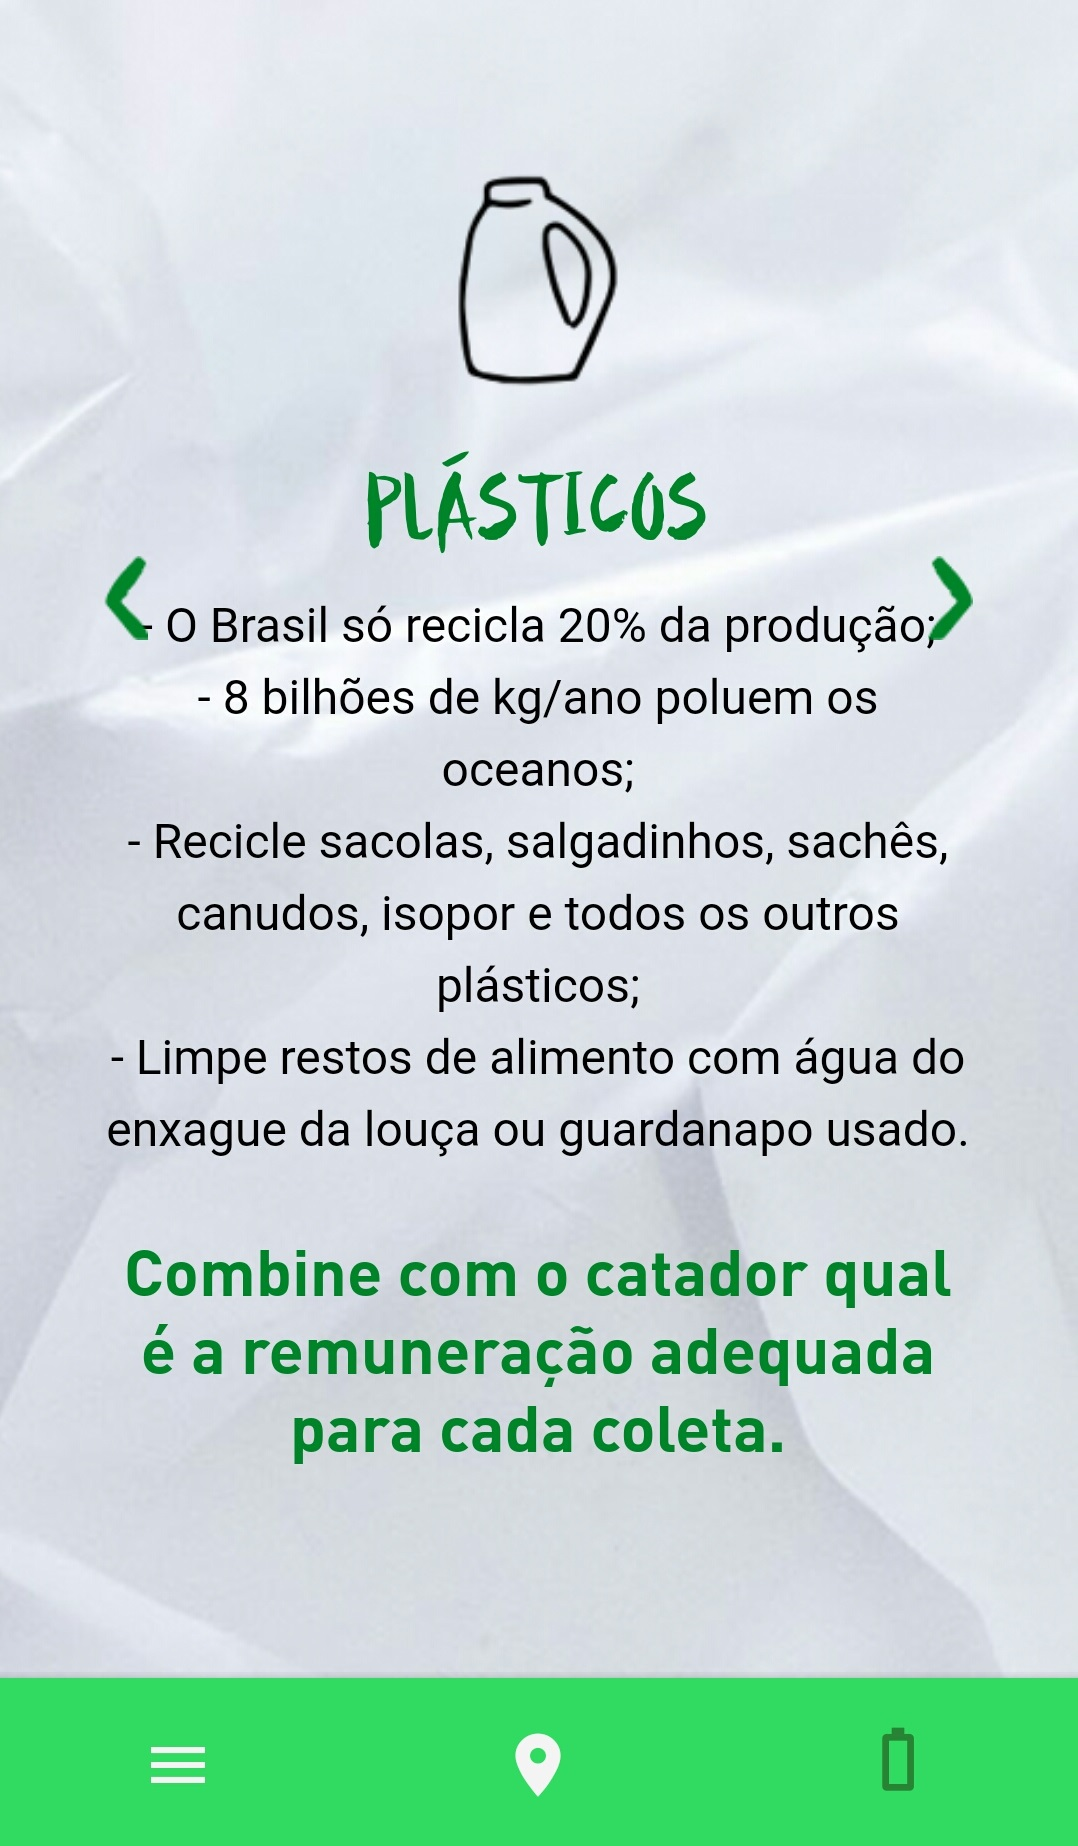
\includegraphics[scale=0.15]{media/catakimateriaisdetalhes.jpg}
    \legend{Fonte: Google Play}
     \label{fig:figura4}
  \end{minipage}
\end{figure}

\section{Recicloteca}

A Recicloteca é um Centro de Informações sobre Reciclagem e Meio Ambiente criado pela ONG Ecomarapendi. Foi desenvolvido com o objetivo de difundir informações sobre as questões ambientais, com ênfase na redução, reaproveitamento e reciclagem de resíduos. Seu acervo é composto pelos mais diversos materiais incluindo livros, vídeos, revistas, periódicos técnico-científicos, cartilhas, teses, produtos reciclados e outros.

Para utilizar a Recicloteca é preciso acessar a pagina na internet \href{http://www.recicloteca.org.br/}{<www.recicloteca.org.br>}, ao acessar a página uma das sessões relevantes para esse trabalho é a sessão de \href{http://www.recicloteca.org.br/pesquisa/}{Pesquisa Escolar} que aparece na página principal, como mostrado na \autoref{fig:reciclotecahome}.

\begin{figure}[h]
\centering
   \caption{Recicloteca - Página Inicial}
   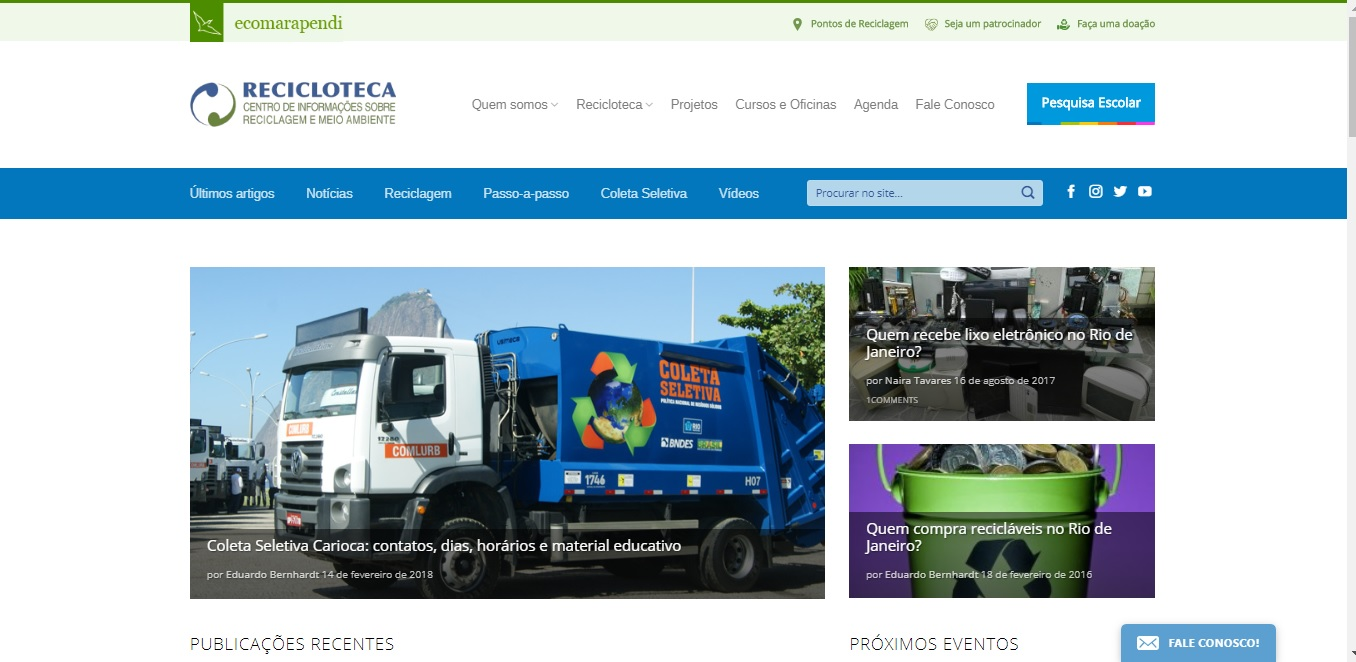
\includegraphics[scale=0.40]{media/reciclotecahome.jpg}
   \legend{Fonte: Recicloteca.org.br}
     \label{fig:reciclotecahome}
\end{figure}

\newpage
Ao clicar em pesquisa escolar, o usuário é redirecionado para uma pagina que contem uma série de vídeos animados separados por diversas categorias, como mostra a \autoref{fig:reciclotecaescola}, esses vídeos são feitos com uma linguagem fácil e uma animação que mantêm o interesse das crianças.


\begin{figure}[h]
\centering
   \caption{Recicloteca - Pesquisa Escolar}
   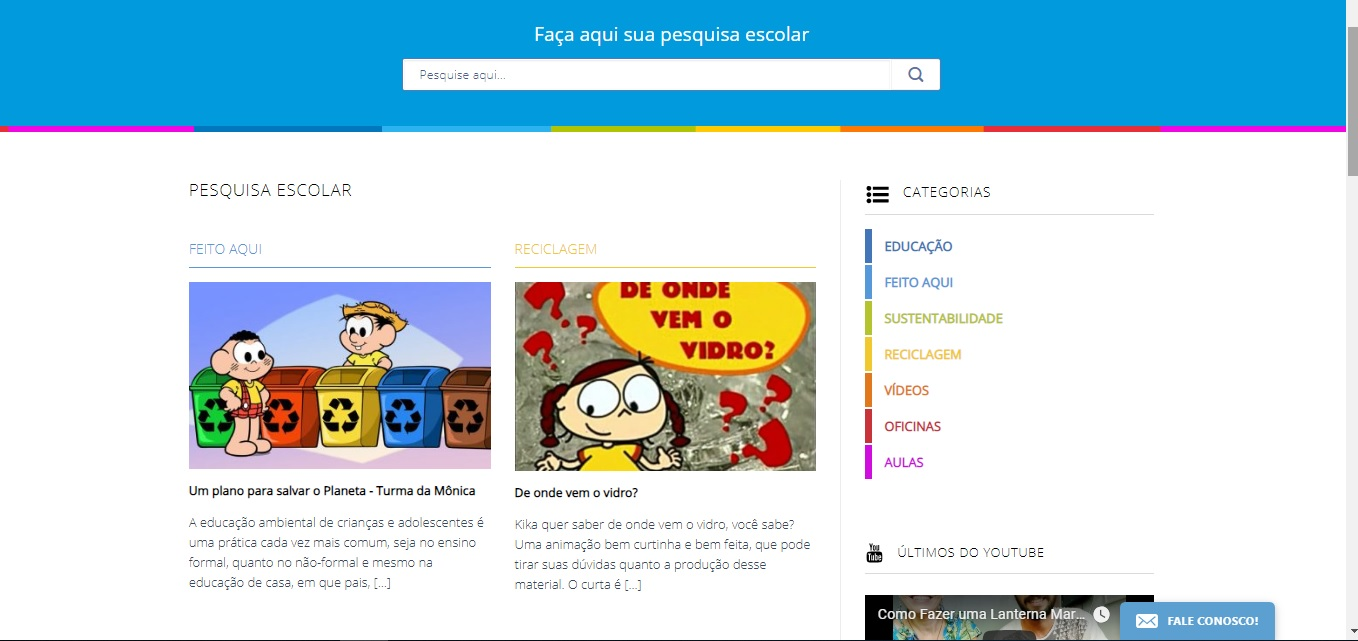
\includegraphics[scale=0.40]{media/reciclotecaescola.jpg}
   \legend{Fonte: Recicloteca.org.br}
     \label{fig:reciclotecaescola}
\end{figure}

\newpage
Outra sessão relevante para esse projeto é a "Passo-a-passo" que pode ser acessada no menu da página principal como mostra a \autoref{fig:reciclotecareciclagem}. Esta sessão contem vídeos e artigos ensinando como reaproveitar itens que seriam descartados dando origem a um novo produto ou a uma nova matéria-prima com o objetivo de diminuir a produção de rejeitos e o seu acúmulo na natureza, reduzindo o impacto ambiental.


\begin{figure}[h]
\centering
   \caption{Recicloteca - Passo-a-passo}
   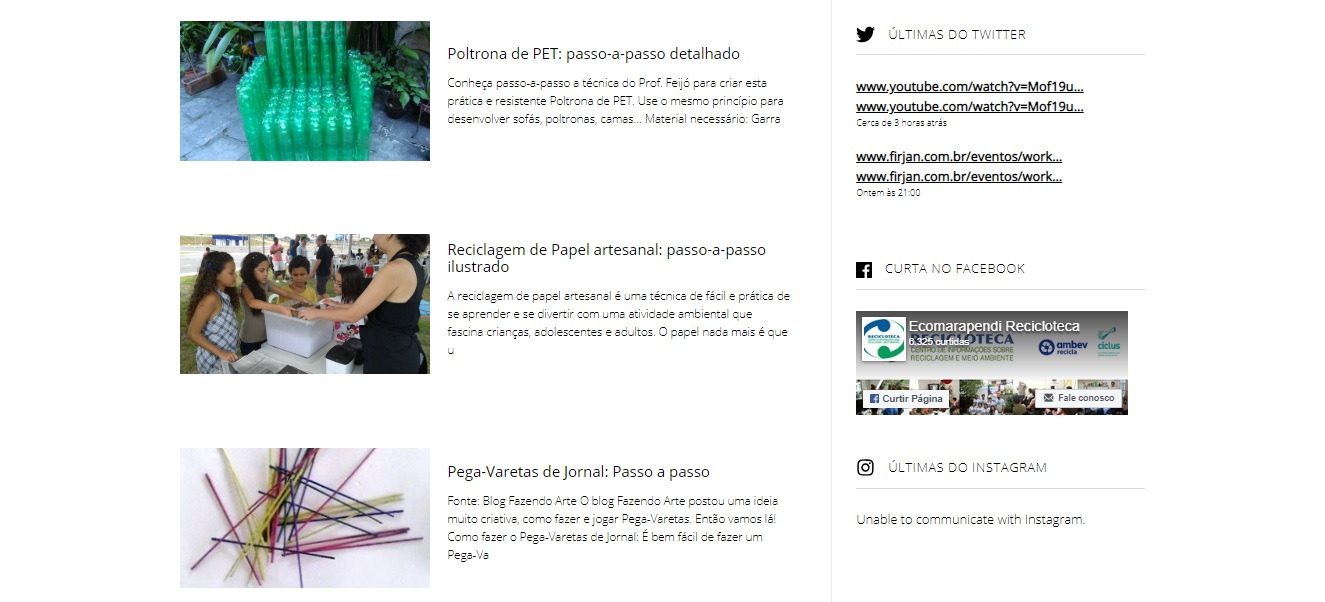
\includegraphics[scale=0.45]{media/reciclotecareciclagem.jpg}
   \legend{Fonte: Recicloteca.org.br}
     \label{fig:reciclotecareciclagem}
\end{figure}


% ---

\newpage
\section{Rota da Reciclagem}

O Rota da Reciclagem é um aplicativo que promove a reciclagem e a defesa do meio ambiente. Este mostra como qualquer pessoa interessada pode participar da separação e entrega das embalagens longa vida para a reciclagem, informando ainda onde estão localizadas as cooperativas de catadores, as empresas comerciais que trabalham com compra de materiais recicláveis e os pontos de entrega voluntária que recebem embalagens da Tetra Pak\cite{tetrapark}.

Para utilizar o aplicativo é preciso efetuar a transferência na Google Play\cite{googleplay} ou na App Store\cite{appstore}, após a transferência basta abrir o aplicativo que apresentará a tela de carregamento. Após o carregamento dos dados uma tela com um campo de texto para inserir o endereço da sua localização aparecerá e ao ser preenchido exibira um mapa mostrando marcadores que representam cooperativas,pontos de entrega, comércios e sua localização atual, como mostra a \autoref{fig:rota2}.
    
    

    
\begin{figure}[htb]    
 \centering
  \begin{minipage}{0.45\textwidth}
    \centering
    \caption{Rota da reciclagem - Tela de carregamento}
    
\includegraphics[scale=0.45]{media/rotaappintro.jpg}   
    \legend{Fonte: Google Play}
     \label{fig:rota1}
  \end{minipage}
  \hfill
  \begin{minipage}{0.45\textwidth}
    \centering
    \caption{Rota da reciclagem - Mapa}
    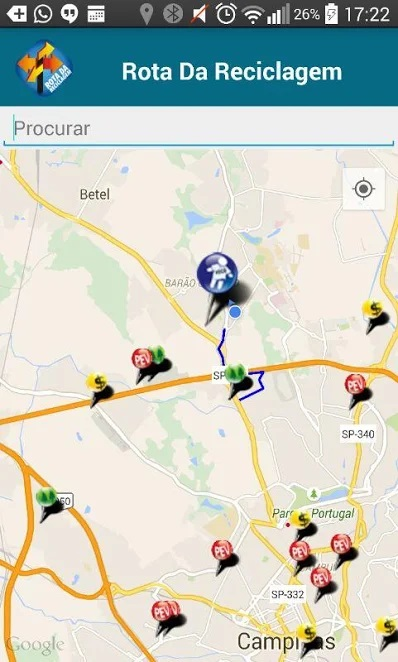
\includegraphics[scale=0.45]{media/rotaappmap.jpg}
    \legend{Fonte: Google Play}
     \label{fig:rota2}
  \end{minipage}
\end{figure}




% ----------------------------------------------------------
\begin{chapter}{Referencial Teórico}
% ----------------------------------------------------------
Neste capítulo serão apresentadas as principais características referentes ao sistema operacional Android e ao desenvolvimento de aplicativos mobile.

\section{Desenvolvimento Mobile}
Existem diversas plataformas de sistemas operacionais mobile em uso nos \textit{smartphones} atuais, grande parte desse mercado é dominado pelas plataformas Android e iOS. Neste projeto utilizaremos a plataforma Android devido a sua alta taxa de adesão.

\begin{figure}[h]
\centering
   \caption{Divisão das plataformas mobile}
   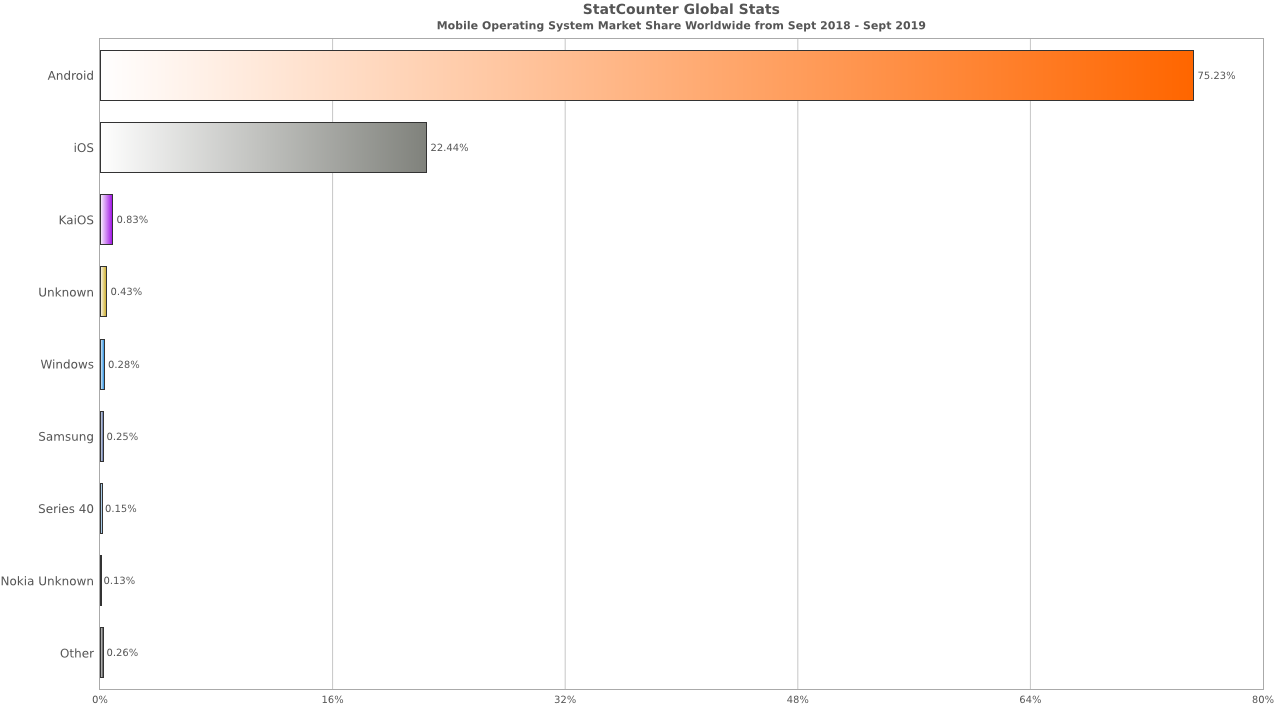
\includegraphics[scale=0.4]{media/grafico_plataformas.png}
   \legend{Fonte: gs.statcounter.com}
     \label{fig:plataformas_mobile}
\end{figure}

\newpage
\section{SDK}
Nessa sessão falaremos dos principais \textit{Software Development Kit} envolvidos no desenvolvimento de aplicativos Android nativo.
\subsection{Android SDK}
O kit de desenvolvimento de software Android (Android SDK) é um pacote com diversas ferramentas utilizadas pelos desenvolvedores parar criar aplicativos para plataforma Android de forma nativa. o SDK inclui as principais bibliotecas, emuladores e ofuscadores.
Embora o SDK possa ser usado por linha de comando, o método mais comum é usar um ambiente de desenvolvimento integrado (IDE). 
\subsection{Java SDK}
O Java SDK, também conhecido como Java Development Kit (JDK) é um conjunto de utilitários que permitem o desenvolvimento de programas capazes de rodar em uma maquina virtual Java (JVM).

\section{Android O.S}
O Google em parceria com outras empresas lançou o desafio de criar um plataforma móvel em que todos os participantes da aliança pudessem utilizar em seus hardwares e que fosse de acesso economicamente viável à população tirando o peso do custo de desenvolvimento de um sistema móvel completo como é, assim nasceu o Android. Uma pilha de softwares para dispositivos móveis que inclui um sistema operacional, um middleware e um conjunto de aplicações chaves. Os desenvolvedores podem criar aplicações para a plataforma usando o Android SDK (Software Development Kit), uma IDE (Integrated Development Environment) e uma linguagem suportada pela SDK. As aplicações para essa plataforma são comumente escritas usando a linguagem de programação Java ou Kotlin.

Os aplicativos gerados são executados sobre o Dalvik ou ART,  máquinas virtuais customizadas para dispositivos com restrições de recursos, como pouca capacidade computacional, baixa capacidade de armazenamento e baterias com baixo nível de energia.

\newpage
\subsection{Arquitetura}
A arquitetura do sistema operacional Android é divida em camadas, onde cada camada é responsável por gerenciar os seus processos. O diagrama na \autoref{fig:arquitetura} mostra essa divisão.

\begin{figure}[h]
\centering
   \caption{Arquitetura Android}
   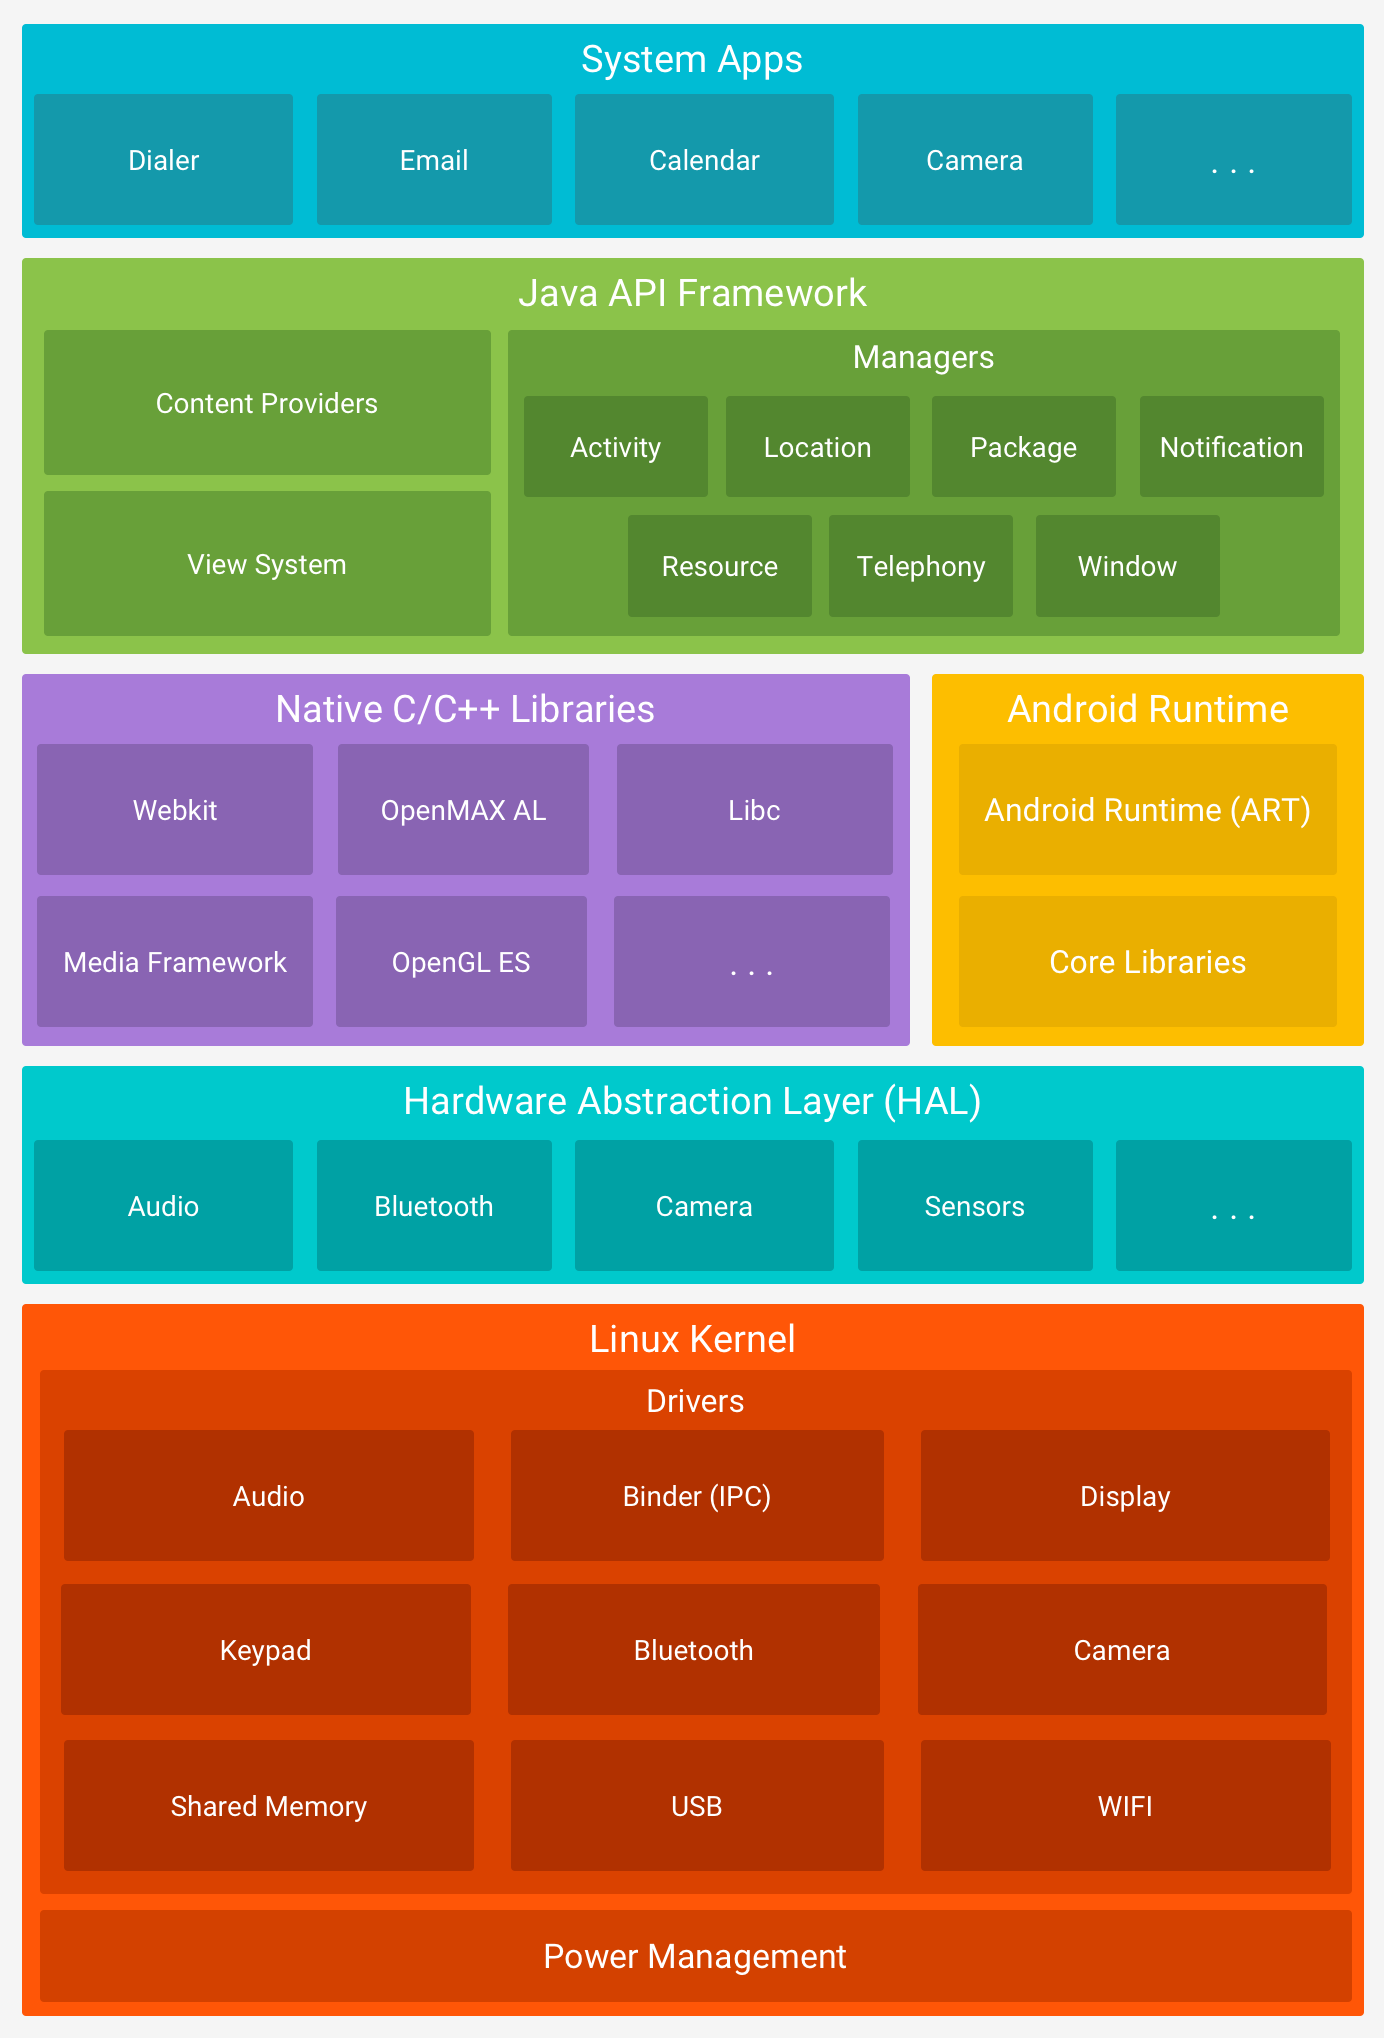
\includegraphics[scale=0.20]{media/android-stack_2x.png}
   \legend{Fonte: developer.android.com}
     \label{fig:arquitetura}
\end{figure}

\newpage

\subsubsection{Kernel}
Os dispositivos móveis possuem arquiteturas distintas e para isso é necessária uma camada capaz de gerenciar os recursos do sistema, além de fornecer aos programas do usuário uma interface simplificada com o hardware.
O sistema operacional Android utiliza o kernel do Linux, que é responsável por gerenciar serviços como segurança, gerenciamento de memória, processos, rede e drivers.

\subsubsection{Android Runtime}
O Android Runtime (ART) é um processo responsável pela compilação de códigos de alto nível (DEX bytecode) em códigos de maquina.
O processo usa uma técnica de compilação chamada AOT (Ahead of Time), sua principal diferença em relação ao Dalvik é que ela ocorre antes 
da execução do aplicativo e não durante a execução. Com isso, há um aumento na velocidade de execução ao custo de um processo que ocupa mais memoria.

\subsubsection{Native C/C++ Libraries}
Vários componentes e diversos serviços do sistema operacional Android são implementados em código nativo,
 o que exige bibliotecas nativas desenvolvidas em C e C++.
O framework Android oferece uma camada de abstração chamada de HAL (Hardware abstraction layer) para expor as funcionalidades de algumas dessas bibliotecas,
 tal abstração permite a manipulação de vídeos, imagens, sons, animações, GPS, etc.

\subsubsection{Java API Framework}
Além das bibliotecas os desenvolvedores tem a sua disposição um conjunto completo de APIs na linguagem java que permitem a interoperabilidade entre aplicativos e subsistemas Android, logo, essas APIs são a base para desenvolvimento de aplicativos Android, facilitando o acesso aos serviços do sistema como gerenciadores de janela, telefone e provedores de conteúdo.

\subsection{Componentes Android}
\subsubsection{Activity} 
É um componente que fornece uma tela a qual o usuário pode interagir, um aplicativo pode ter várias activities de entrada que podem chamar inúmeras activities dependendo da interação do usuário. Para usa-las de forma correta, é necessário entender conceitos como seu ciclo de vida, gerenciamento na memória e seus métodos. 

\subsubsection{Fragment}
Esse componente permite a criação de interfaces ou módulos de interface reutilizáveis, esse componente só existe dentro de uma \textit{activity}, logo, apesar de possuir seu próprio ciclo de vida, alterações no ciclo da vida da \textit{activity} afetam o ciclo de vida do \textit{fragment}.  

\subsection{Gerenciamento de memória}
Em aplicativos moveis os recursos do sistema são fatores importantes para garantir o desempenho de todas as aplicações, por isso, o sistema operacional \textit{Android} controla como seus recursos serão distribuídos. Aplicativos que estão abertos em segundo plano ou \textit{activities} empilhadas podem ter telas destruídas e variáveis removidas da memoria a qualquer momento. Para solucionar esse problema o sistema operacional oferece um conjunto de \textit{callbacks} no componente \textit{activity} para que o desenvolvedor possa controlar os comportamentos durante as mudanças de estado do sistema, esses estados são controlados pelo ciclo de vida.

\begin{figure}[h]
\centering
   \caption{Empilhamento de activities}
   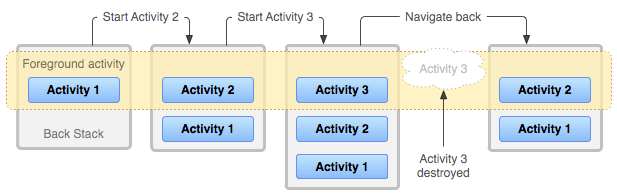
\includegraphics[scale=0.70]{media/diagram_backstack.png}
   \legend{Fonte: developer.android.com}
     \label{fig:backstack}
\end{figure}

\subsection{Ciclo de vida}
À medida que o usuário navega no aplicativo, sai dele e retorna a ele, as instâncias \textit{Activity} no aplicativo transitam entre diferentes estados no ciclo de vida. A classe Activity fornece uma quantidade de \textit{callbacks} que permite que o desenvolvedor saiba sobre a mudança do estado.

O Diagrama a seguir mostra quando os \textit{callback} são executados durante a mudança do ciclo de vida da \textit{activity}.
\begin{figure}[h]
\centering
   \caption{Ciclo de vida - Activity}
   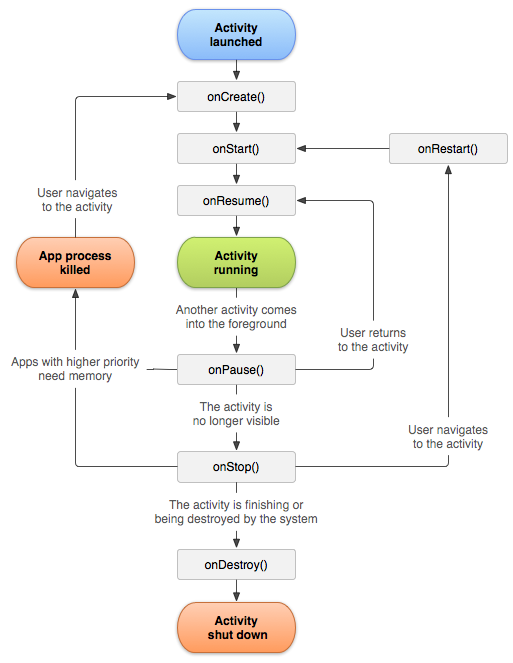
\includegraphics[scale=0.70]{media/activity_lifecycle.png}
   \legend{Fonte: developer.android.com}
     \label{fig:lifecycle}
\end{figure}

\newpage
\begin{itemize}
\item{OnCreate} \\
     É chamado assim que uma \textit{activity} é iniciada, boa parte da inicialização é feita nesse \textit{callback}, incluindo o processo de inflação da interface de usuário. O \textit{onCreate} é executado uma vez durante a inicialização e só será chamado novamente caso o sistema operacional decida destruir a \textit{activity} para liberar recursos para \textit{activities} com maior prioridade.
     \item{OnStart} \\
     Chamado após o \textit{OnCreate} ou após o \textit{OnRestart}, o \textit{Onstart} é executado quando a interface gráfica está visível, porem o usuário ainda não pode interagir. Esse \textit{callback} é normalmente utilizado inicializações adicionais, desenhar componentes e executar animações.
     \item{OnResume} \\
      Chamado quando a atividade vai iniciar a interação com o usuário. Nesse ponto, sua atividade está no topo da pilha de atividades.
      \item{OnRestart} \\
      Chamada após o \textit{OnStop} quando uma \textit{activity} que está na pilha é recriada.
     \item{OnPause} \\
     Chamado quando o sistema está por resumir a \textit{activity} anterior. É tipicamente usado para persistir mudanças ainda não efetivadas, parar animações e liberar recursos. A partir desse ponto o sistema operacional pode forçar a liberação de recursos consumidos pela \textit{activity} pausada.
     \item{OnStop} \\
    Chamado quando a \textit{activity} não está mais visível para o usuário. Isso pode acontecer porque ela está sendo destruída ou porque outra  \textit{activity} foi reiniciada e está em sua frente. Aqui é o lugar para liberar todos os recursos que não são mais utilizados pelo usuário.
     \item{OnDestroy} \\
     Chamado quando a \textit{activity} vai ser destruída. É a última chamada que a \textit{activity} receberá antes de ser finalizada.
  \end{itemize}

\newpage
\section{API}
A \textit{Application Programming Interface} (API) permite a comunicação e consumo de dados entre aplicações. Um dos motivos que tornam o uso de uma \textit{API} atrativo é a abstração, já que não é necessário conhecer a plataforma ou maneira que o aplicativo consumidor foi desenvolvido. Outra vantagem é o fato deste modelo ser baseado em tecnologias padrões, em particular o HTTP (Hypertext Transfer Protocol). Os dados transferidos entres essas aplicações seguem um formato padrão, os mais utilizados são \textit{JavaScript Object Notation} (JSON) e \textit{Extensible Markup Languag} (XML). Neste projeto utilizaremos JSON no desenvolvimento de API.

\section{JSON}
\textit{JavaScript Object Notation} (JSON) é um formato leve de troca de dados entre sistemas independente de linguagem de programação. O formato foi derivado do JavaScript, sendo fácil para humanos ler e escrever.

\section{Firebase}
\subsection{Firebase Realtime Database}
O \textit{Firebase Realtime Database} é um banco de dados NoSQL hospedado na nuvem, com ele, você armazena os dados em um formato JSON e sincroniza dados entre os seus usuários em tempo real, permitindo que os dados continuem disponíveis quando o aplicativo estiver off-line.

\subsection{Firebase Authentication}
O objetivo do \textit{Firebase Authentication} é facilitar o desenvolvimento de um sistema de autenticação seguro e melhorar a experiência de login e ambientação para os usuários finais. Ele oferece uma solução de identidade completa, compatível com contas de e-mail/senha, autenticação por telefone, login do Google, Twitter, Facebook, GitHub e outros.

\end{chapter}
\begin{chapter}{Projeto}
Neste capítulo serão apresentadas as instalações e configurações iniciais das ferramentas e bibliotecas utilizadas no desenvolvimento de aplicativos Android
\section{Instalação}
Nesta sessão será abordado os  recursos necessários para iniciar o desenvolvimento desse projeto.
\begin{enumerate}
  \item{Android Studio} \\
  Neste projeto usaremos o Android Studio, IDE recomendada pela Google para o desenvolvimento de aplicativos nativos. O Android Studio está disponível em \url{https://developer.android.com/studio/install}.
  \item{SDK e JDK} \\ Para iniciar o desenvolvimento Android foi instalado o Android SDK, que por sua vez necessita do JDK, já que o código gerado pelo SDK roda em uma maquina virtual Java customizada, a ART.
  O JDK esta disponível em \url{https://www.oracle.com/technetwork/java/javase/downloads/index.html} e o SDK em \url{https://developer.android.com/studio}.
  \item{GIT} \\
  Para realizar o controle de versão do aplicativo usaremos o GIT, um sistema de controle de versões distribuído, usado principalmente no desenvolvimento de software, mas pode ser usado para registrar o histórico de edições de qualquer tipo de arquivo. 
  GIT está disponível em \url{https://www.git-scm.com/}.
  
\end{enumerate}






\section{Configuração}
\subsection{Gradle}
Gralde é um sistema de automação de compilação de código aberto utilizado para configuração de projetos. Foi projetado para suportar \textit{builds}\footnote{Processo de compilação de um programa} incrementais e determinar que partes do projeto precisam ser atualizadas, atualizando somente as dependências necessárias.
No projeto Android, o arquivo de configuração do Gradle pode ser encontrado no diretório abaixo. \begin{lstlisting}[
    basicstyle=\small,
]
/app/build.gradle
\end{lstlisting}
\subsubsection{Dependências}
 No build.gradle, o campo \textit{dependencies} nos permite baixar bibliotecas externas, adicionar arquivos jar ou módulos em nosso projeto Android. Neste projetos utilizaremos as dependências abaixo.
 
   \paragraph{Google Play Services}
   As bibliotecas criadas pela Google disponiveis em \url{https://developers.google.com/android/guides/setup}, oferecem aos desenvolvedores os últimos recursos e funcionalidades mantidas pela Google, como por exemplo, GPS e mapas.
       \begin{lstlisting}[
    basicstyle=\small,
] 
implementation 'com.google.android.gms:play-services-maps:15.0.1'
implementation 'com.google.android.gms:play-services-location:15.0.1'
implementation 'com.google.android.gms:play-services-places:15.0.1'
  
\end{lstlisting}
   \paragraph{Volley}
   Também desenvolvida pela Google, disponível em \url{https://github.com/google/volley}, Volley é uma biblioteca que permite realizar requisições HTTP de forma simplificada, sem a necessidade de criação de chamadas assíncronas.
       \begin{lstlisting}[
    basicstyle=\small,
]
implementation 'com.android.volley:volley:1.1.0'  
\end{lstlisting}

\paragraph{Lottie}
\label{Lottie}

   \paragraph{MPAndroidChart}
   A  MPAndoridChart disponível em \url{https://github.com/PhilJay/MPAndroidChart} é uma poderosa biblioteca que simplifica a criação de diversos tipos de gráficos. 
        \begin{lstlisting}[
    basicstyle=\small,
] 
implementation 'com.github.PhilJay:MPAndroidChart:v3.0.3'
  
\end{lstlisting}
   \paragraph{Firebase}
O Firebase, disponível em \url{https://firebase.google.com} é um conjunto de soluções criadas pela Google para agilizar e melhorar o desenvolvimento de aplicações. Neste projeto usaremos somente o \textit{Firebase Realtime Database} , que é um banco de dados hospedado na nuvem. Os dados são armazenados como JSON e sincronizados em tempo real com todos os clientes conectados
        \begin{lstlisting}[
    basicstyle=\small,
]
implementation 'com.google.firebase:firebase-database:16.0.1'
  
\end{lstlisting}
\newpage
   \paragraph{Glide}
   disponível em \url{https://github.com/bumptech/glide}, Glide é uma biblioteca de gerenciamento e carregamento de imagens 
que simplifica tarefas como decodificação, cache em memoria e em disco. 
        \begin{lstlisting}[
    basicstyle=\small,
]
implementation 'com.github.bumptech.glide:glide:4.7.1'
  
\end{lstlisting}
   \paragraph{SmartTabLayout}
   A biblioteca SmartTabLayout disponível em \url{https://github.com/ogaclejapan/SmartTabLayout}, fornece uma implementação mais customizável 
para criação de menus em componentes do sistema operacional Android.
         \begin{lstlisting}[
    basicstyle=\small,
]
implementation 'com.ogaclejapan.smarttablayout:library:1.6.1@aar'
   
\end{lstlisting}
        \begin{lstlisting}[
    basicstyle=\small,
]
implementation 'com.ogaclejapan.smarttablayout:utils-v4:1.6.1@aar'
   
\end{lstlisting}
   \paragraph{Gson}
   Desenvolvida pela Google, disponível em \url{https://github.com/google/gson}, Gson é uma biblioteca que pode ser usada para converter objetos Java (POJO) em representações JSON ou vice-versa.
         \begin{lstlisting}[
    basicstyle=\small,
]
implementation 'com.google.code.gson:gson:2.8.5'
    
\end{lstlisting}
   \paragraph{YouTubeAndroidPlayerApi}
   Desenvolvida pela Google, disponível em \url{https://developers.google.com/youtube/android/player}, YouTubeAndroidPlayerApi permite incorporar a funcionalidade de reprodução de video em aplicativos Android. A API  define métodos para carregar, reproduzir 
e controlar a experiência de reprodução de vídeo.
      \begin{lstlisting}[
    basicstyle=\small,
]
implementation files('libs/YouTubeAndroidPlayerApi.jar')
   
\end{lstlisting}
   \paragraph{Fabric}
   A biblioteca Fabric, também conhecida como Crashlytics, disponível em \url{https://fabric.io/kits/android/crashlytics/install}, ajuda a rastrear, priorizar e corrigir problemas de instabilidade que podem prejudicar a qualidade do aplicativo e a experiencia do usuário.
   \begin{lstlisting}[
    basicstyle=\small,
]
implementation 'com.crashlytics.sdk.android:crashlytics:2.9.9'
   
\end{lstlisting}

\newpage

\section{Desenvolvimento}
Nesta sessão, serão abordadas as etapas do desenvolvimento da solução proposta nesse documento, desde a criação do subsistema que irá gerenciar todo conteúdo até o aplicativo Android. 

\subsection{Arquitetura Geral}
Para possibilitar a entrega de conteúdo dinâmica no aplicativo, foi escolhida uma arquitetura cliente-servidor onde o aplicativo consome dados em servidores da Google através de uma API ou SDK. Esses servidores são populados com informações relevantes ao aplicativo através de uma pagina \textit{web} administrativa. O processo de desenvolvimento dessa pagina será abstraído neste documento.\\


\begin{figure}[h]
\centering
   \caption{Arquitetura geral}
   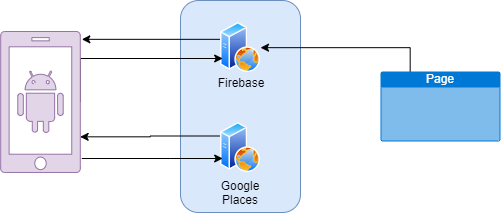
\includegraphics[scale=0.85]{media/arquitetura_app.png}
   \legend{Fonte: Autor}
     \label{fig:arquitetura_geral}
\end{figure}

\subsection{Arquitetura do Aplicativo}
\textit{Model-View-Controller} (MVC),  \textit{Model-View-Presenter} (MVP) e \textit{Model-View-ViewModel} (MVVM) são três padrões de arquitetura populares no desenvolvimento de aplicativos Android. Todos esses padrões de arquitetura ajudam os desenvolvedores a desenvolver aplicativos fracamente acoplados, fáceis de testar e manter. o Padrão MVC é usado em projetos de pequeno porte, pois o possui um acoplamento maior do que os outros padrões como MVP e MVVM, que são padrões para projetos de médio e grande porte respectivamente. Neste projeto usaremos MVC.\\

\subsubsection{MVC}
A arquitetura MVC consiste na divisão do aplicativo em três camadas,  \textit{model}, \textit{view} e \textit{controller}. Por questões da arquitetura do sistema operacional Android e sua SDK, não é possível implementar um padrão arquitetural MVC da forma convencional, pois \textit{fragments} e \textit{activities} assumem papeis da camada \textit{controller} e \textit{view} simultaneamente.

\begin{itemize}
  \item{Model}\\ Essa camada fica responsável pelo acesso aos repositórios para salvar e entregar dados a camada controladora.
     \item{View}\\ Essa camada fica responsável pela apresentação da interface gráfica.
       \item{Controller}\\ A camada \textit{controller} é responsável por implementar as regras de negocio e fornecer os dados do modelo para a camada \textit{view}. Quaisquer alterações ao controlador são transparentes para a \textit{view} e as mudanças de interface do usuário não afetarão a lógica de negócios e vice-versa.
\end{itemize}

\begin{figure}[h]
\centering
   \caption{Arquitetura do aplicativo}
   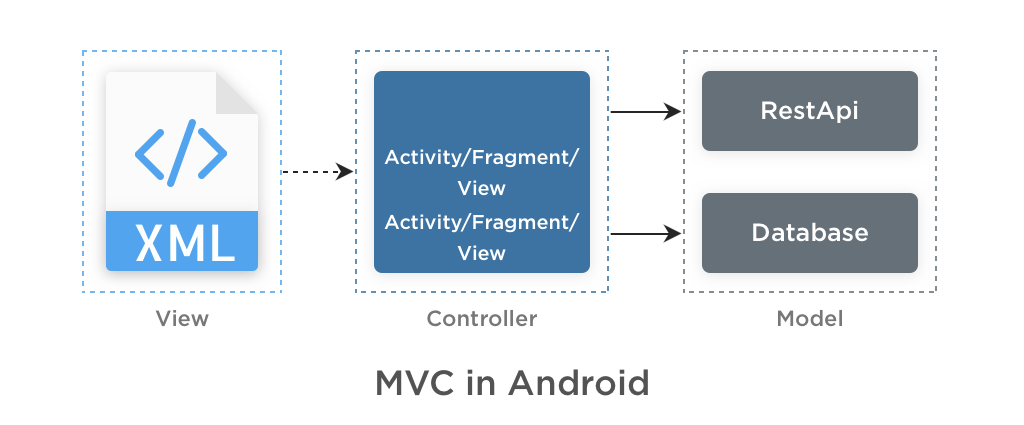
\includegraphics[scale=0.40]{media/MVC.png}
   \legend{Fonte: www.simform.com}
     \label{fig:arquitetura_mvc}
\end{figure}


\subsection{Banco de dados}
Para a prestância da dados foi escolhido o banco de dados mais popular entre os desenvolvedores mobile, o \textit{Firebase Realtime Database}. O \textit{Firebase}, através da sua SDK, oferece um desenvolvimento simplificado, facilitando processos comuns em aplicações \textit{mobile}, como autenticação, leitura e escrita de dados.
 Os diagramas a seguir representam as entidades que serão utilizadas neste projeto.


\subsubsection{Entidades}
\begin{enumerate}
 \item{Material} \\ A classe \textit{MaterialModel} representa a estrutura de um material reciclável, como por exemplo, ferro, plástico e papel. Esta classe possui os seguintes atributos:
 
 \begin{itemize}
  \item{Cod}\\ Identificador único do material.
   \item{PopularName}\\ Nome popular do material.
     \item{Name}\\ Nome cientifico do material.
       \item{Content}\\ informações detalhadas do material.
         \item{Type}\\ Tipo de material
           \item{Image}\\ Imagem ilustrativa do material.
\end{itemize}
  
\begin{figure}[h]
\centering
   \caption{Entidade - Material}
   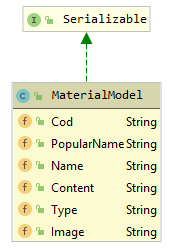
\includegraphics[scale=1.0]{media/materialModel.png}
   \legend{Fonte: Autor}
     \label{fig:materialmodel}
\end{figure}


  \item{Video}  \\ A classe \textit{VideoModel} representa a estrutura de um video que será disponibilizado através de uma \textit{url} do \textit{YouTube}. Esta classe possui os seguintes atributos:
   \begin{itemize}
  \item{Cod}\\ Identificador único do video.
   \item{Url}\\ Endereço do video no YouTube.
     \item{Title}\\ Titulo do video que será apresentado no aplicativo.
       \item{Description}\\ Descrição do video que será apresentado no aplicativo.
         \item{Page}\\  O identificador único da pagina em que será apresentado o video.
\end{itemize}
  
\begin{figure}[h]
\centering
   \caption{Entidade - Video}
   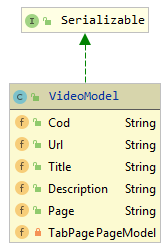
\includegraphics[scale=1.0]{media/VideoModel.png}
   \legend{Fonte: Autor}
     \label{fig:videomodel}
\end{figure}


  \item{Product} \\ A classe \textit{ProductModel} representa a estrutura de um produto, como por exemplo, telefones, brinquedos e produtos descartáveis em geral. Esta classe possui os seguintes atributos:
  
     \begin{itemize}
  \item{Cod}\\ Identificador único do produto.
     \item{Title}\\ Titulo ou nome do produto.
       \item{Desc}\\ Descrição do produto.
         \item{Synonymous}\\ Nomes alternativos do produto.
                  \item{Discard}\\ Identificador único de um tipo de descarte.
\end{itemize}
  
\begin{figure}[h]
\centering
   \caption{Entidade - Product}
   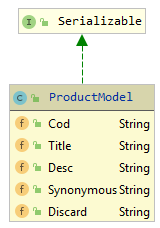
\includegraphics[scale=1.0]{media/ProductModel.png}
   \legend{Fonte: Autor}
     \label{fig:productModel}
\end{figure}


  \item{Location}  \\ A classe \textit{LocationModel} representa a estrutura de uma localização no mapa, como por exemplo, centros de reciclagem, lixões e aterros. Esta classe possui os seguintes atributos:
  
       \begin{itemize}
  \item{UniqueID}\\ Identificador único de uma localização.
     \item{FormattedAddress}\\ O endereço formatado de um local.
       \item{Name}\\ Nome do local.
         \item{Location}\\ Posição baseada no sistema de posicionamento global (GPS), com latitude e longitude.
\end{itemize}
  
  
\begin{figure}[h]
\centering
   \caption{Entidade - Location}
   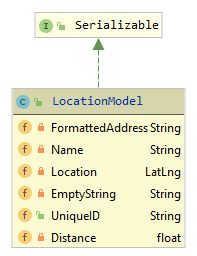
\includegraphics[scale=0.85]{media/LocationModel.png}
   \legend{Fonte: Autor}
     \label{fig:locationModel}
\end{figure}


  \item{Chart}   \\ A classe \textit{ChartModel} representa a estrutura de um gráfico do tipo \textit{PieChart} ou \textit{BarChart}. Esta classe possui os seguintes atributos:
  
  \begin{itemize}
  \item{UniqueID}\\ Identificador único de um gráfico.
     \item{Data}\\ Um conjunto pré formatado de dados a serem inseridos no gráfico.
       \item{Label}\\ Etiquetas que descreve os dados apresentados no gráfico.
         \item{Type}\\ O tipo de gráfico.
         \item{Title}\\ O titulo do gráfico.
         \item{Page}\\  O identificador único da pagina em que será apresentado o gráfico.
\end{itemize}
  
\begin{figure}[h]
\centering
   \caption{Entidade - Chart}
   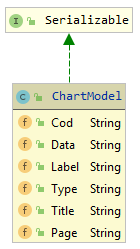
\includegraphics[scale=1.0]{media/chartModel.png}
   \legend{Fonte: Autor}
     \label{fig:chartModel}
\end{figure}


  \item{Discard}   \\ A classe \textit{DiscardModel} representa a estrutura de um método de descarte de materiais, por exemplo, lixão, aterro e centro de reuso. Esta classe possui os seguintes atributos:
  
  \begin{itemize}
  \item{Cod}\\ Identificador único de um gráfico.
       \item{Title}\\Titulo do tipo descarte.
         \item{Desc}\\ Descrição do tipo de descarte.
  
    
\end{itemize}
  
\begin{figure}[h]
\centering
   \caption{Entidade - Discard}
   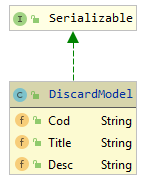
\includegraphics[scale=1.0]{media/discardModel.png}
   \legend{Fonte: Autor}
     \label{fig:discardModel}
\end{figure}

  \item{Page}   \\ A classe \textit{PageModel} representa a estrutura de uma página que pertence a uma categoria. Esta classe possui os seguintes atributos:
  \begin{itemize}
  \item{Cod}\\ Identificador único de um gráfico.
       \item{Number}\\Número da pagina.
         \item{Type}\\ Categoria da página
         . \item{Type}\\ Título da página
\end{itemize}
\begin{figure}[h]
\centering
   \caption{Entidade - Page}
   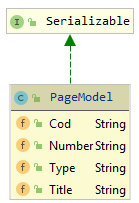
\includegraphics[scale=1.0]{media/PageModel.png}
   \legend{Fonte: Autor}
     \label{fig:pageModel}
\end{figure}

\item{DataWrapper}   \\ A classe \textit{DataWrapper} engloba todos os dados que serão utilizados na aplicação, essa classe foi criada para facilitar a requisição de dados em uma única requisição ao servidor. Vale ressaltar que dados como imagens e vídeos são enviados para o aplicativo de acordo com a necessidade, logo, não há sobrecarga ao realizar uma única requisição.
\newline
  \begin{itemize}
  \item{GraphList}\\ Todos os gráficos .
       \item{PageList}\\  Todas as páginas 
         \item{VideoList}\\ Todos os vídeos
         . \item{LocationList}\\ Todas as localizações pesquisadas pelo usuario.
         \item{ProductList}\\  Todos os produtos
         \item{DiscardList}\\ Todos os métodos de descarte 
         \item{MaterialList}\\  Todos os materiais
         
\end{itemize}
\begin{figure}[h]
\centering
   \caption{Entidade - DataWrapper}
   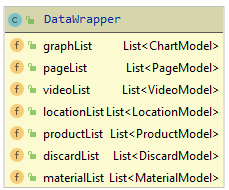
\includegraphics[scale=1.0]{media/DataWrapperModel.png}
   \legend{Fonte: Autor}
     \label{fig:datawrapper}
\end{figure}
\end{enumerate}

\newpage
\subsubsection{Diagrama de classe geral}
As imagens a seguir representam as dependências entre as entidades.

\begin{figure}[h]
\centering
   \caption{Diagrama Geral - Simplificado}
   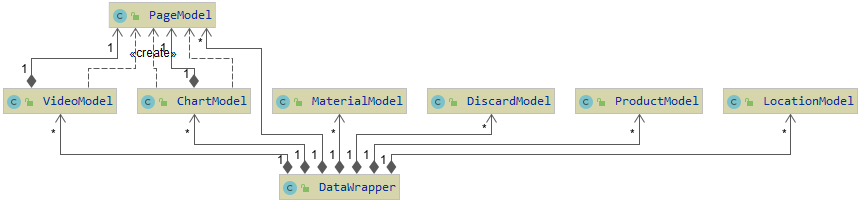
\includegraphics[scale=0.7]{media/DataWrapper_.png}
   \legend{Fonte: Autor}
     \label{fig:datawrapper_simp}
\end{figure}

\begin{figure}[h]
\centering
   \caption{Diagrama Geral - Completo}
   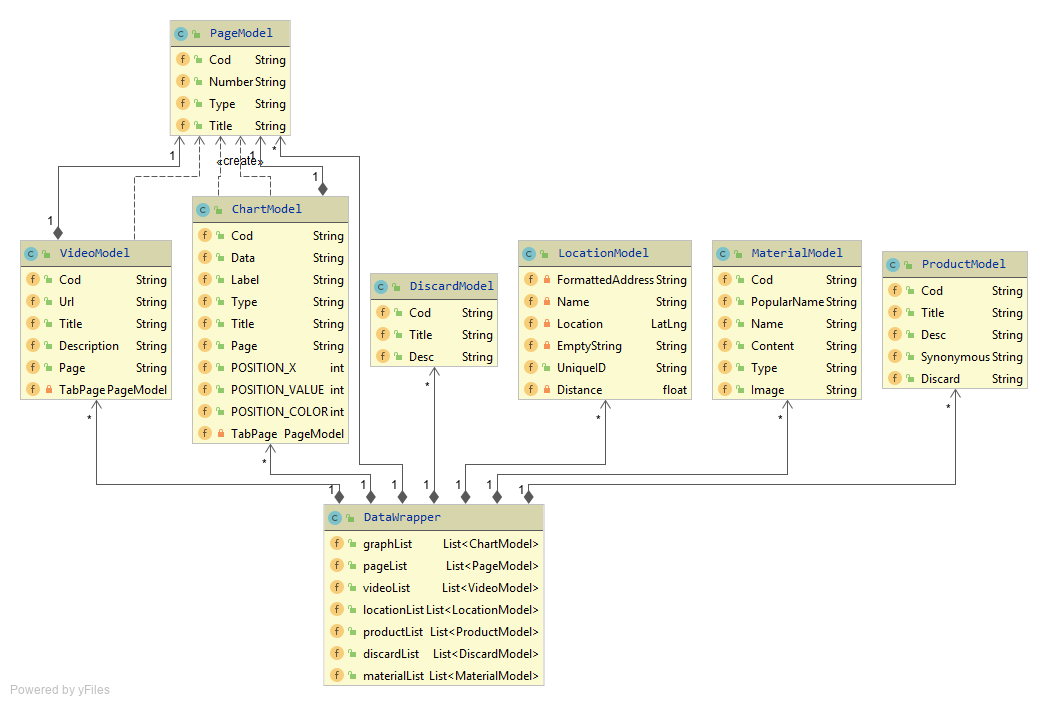
\includegraphics[scale=0.85]{media/DataWrapper.png}
   \legend{Fonte: Autor}
     \label{fig:datawrapper_comp}
\end{figure}

\newpage
\subsection{Sistema Administrativo}
Para disponibilizar dados para o aplicativo mobile foi desenvolvido um sistema administrativo responsável por inserir ou modificar o conteúdo exibido. O sistema foi desenvolvido usando tecnologias web, como HTML, Javascript e CSS. Nesta sessão sera abordado as principais funcionalidades do sistema, abstraindo a implementação.
\subsubsection{Tela de autenticação}
Para controlar o acesso ao sistema foi desenvolvido um sistema de autenticação por e-mail utilizando o \textit{firebase authentication}, dessa forma somente usuários cadastrados e com perfis de acesso podem realizar alterações e inclusões de conteúdo pelo sistema administrativo. 
A alteração e inclusão de novos usuários é feita diretamente pelo painel administrativo do \textit{firebase}.


\begin{figure}[h]
\centering
   \caption{Tela de autenticação}
   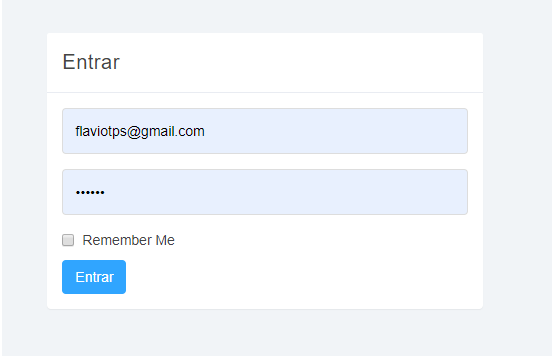
\includegraphics[scale=0.85]{media/tela_login_site_1.png}
   \legend{Fonte: Autor}
     \label{fig:tela_login_site_1}
\end{figure}

\newpage
\subsubsection{Tela de materiais}
A tela de materiais é responsável por inserir e modificar materiais recicláveis, como por exemplo, plástico, metais e papeis. As informações do material podem ser escritas em HTML, tornando menu mais flexível.
\begin{figure}[h]
\centering
   \caption{Material - Todos}
   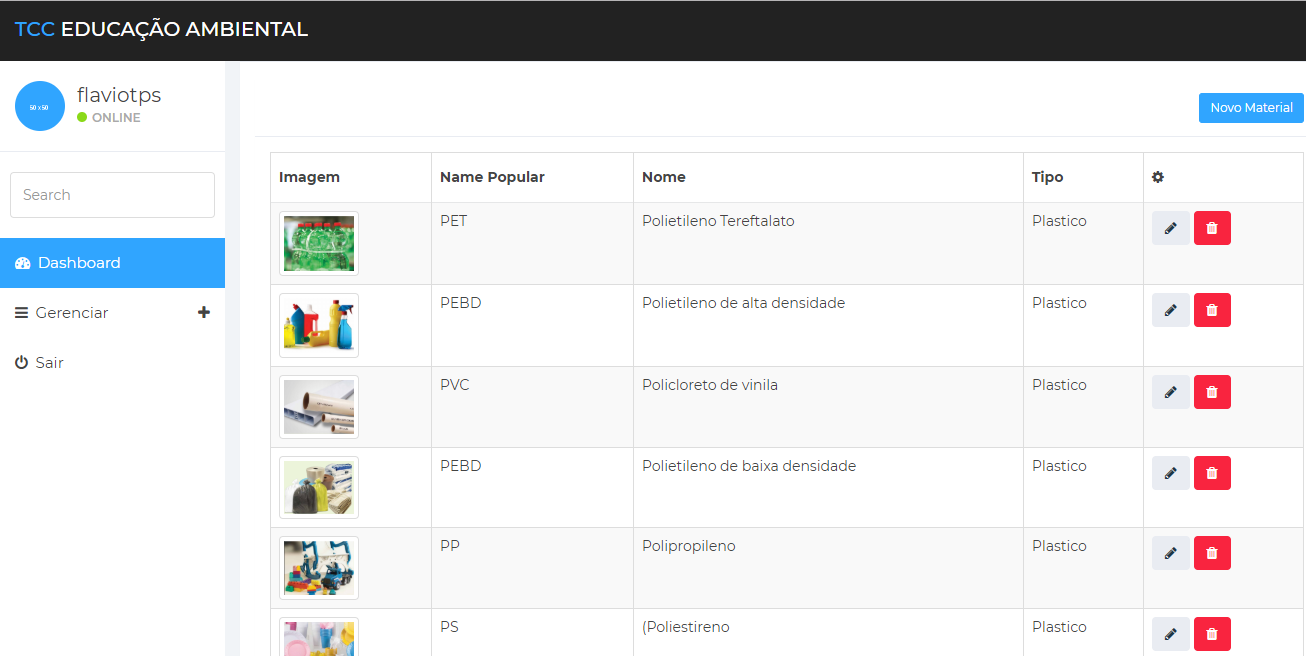
\includegraphics[scale=0.45]{media/tela_material_site_1.png}
   \legend{Fonte: Autor}
     \label{fig:tela_material_site_1}
\end{figure}

\begin{figure}[h]
\centering
   \caption{Material - Edição}
   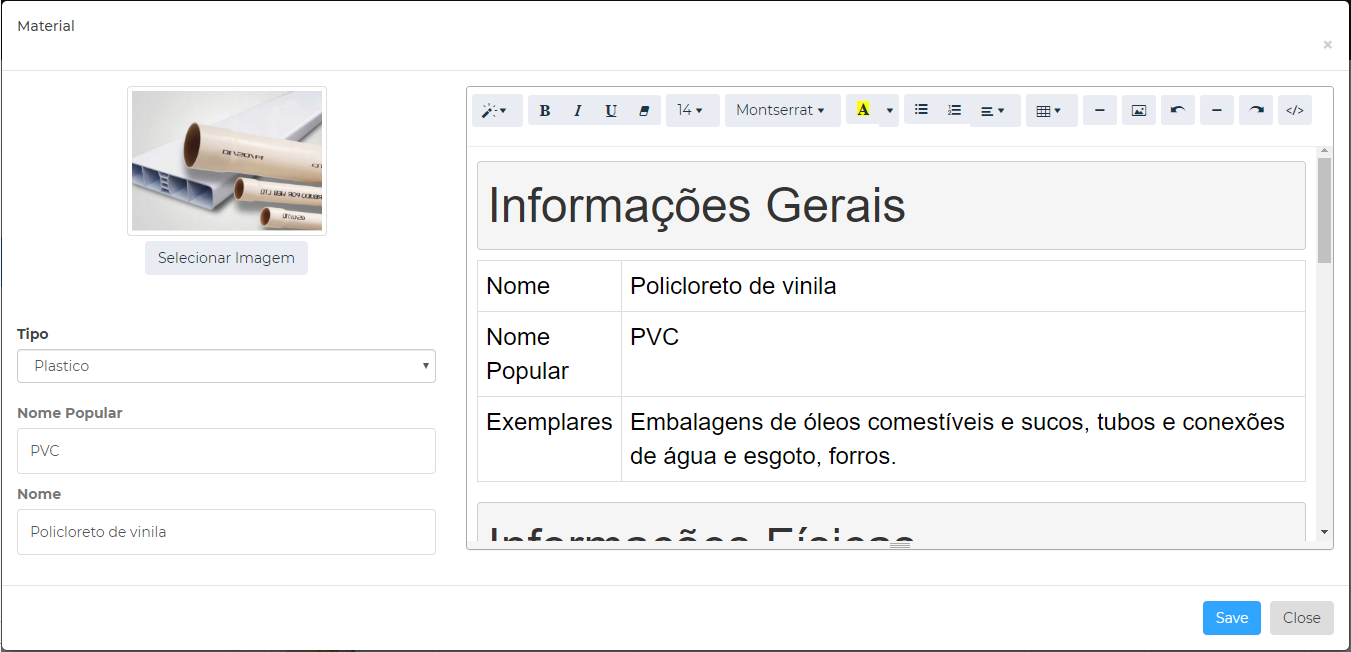
\includegraphics[scale=0.40]{media/tela_material_site_2.png}
   \legend{Fonte: Autor}
     \label{fig:tela_material_site_2}
\end{figure}

\newpage
\subsubsection{Tela de produtos}
A área de produtos permite adicionar produtos de uso diário, como por exemplo, telefones, brinquedos e utensílios domésticos. 

\begin{figure}[h]
\centering
   \caption{Produto - Todos}
   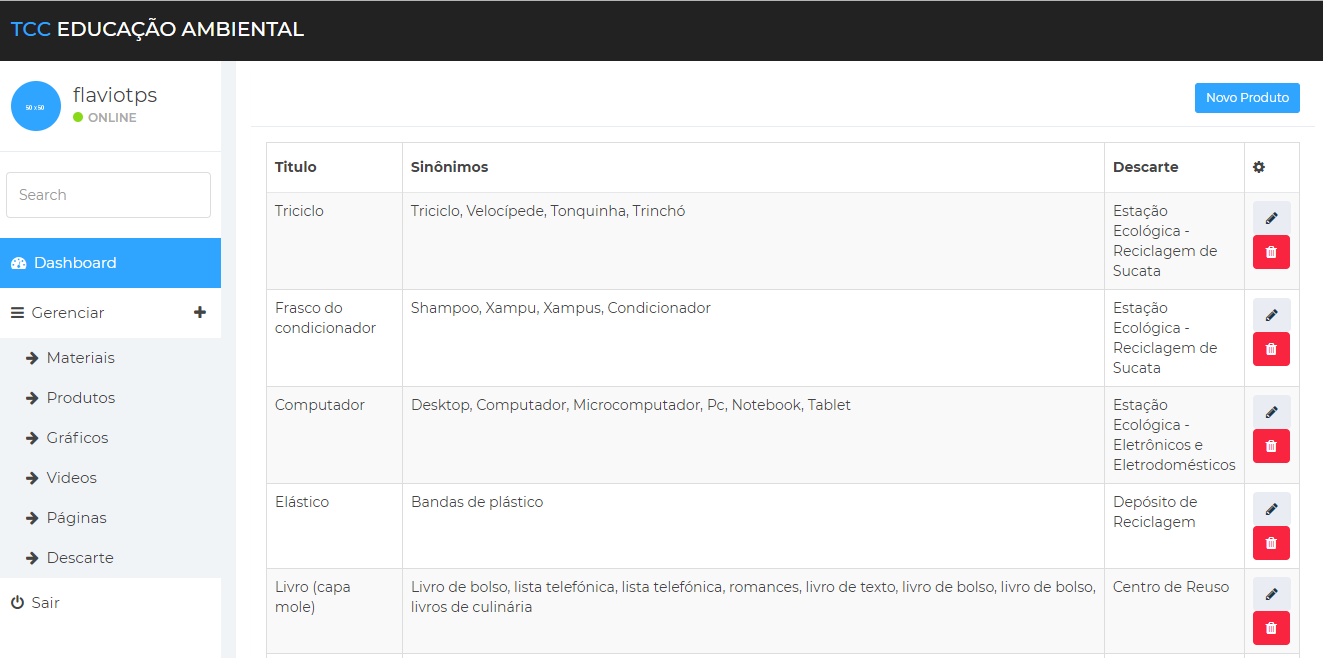
\includegraphics[scale=0.45]{media/tela_produto_site_1.png}
   \legend{Fonte: Autor}
     \label{fig:tela_produto_site_1}
\end{figure}

\begin{figure}[h]
\centering
   \caption{Produto - Edição}
   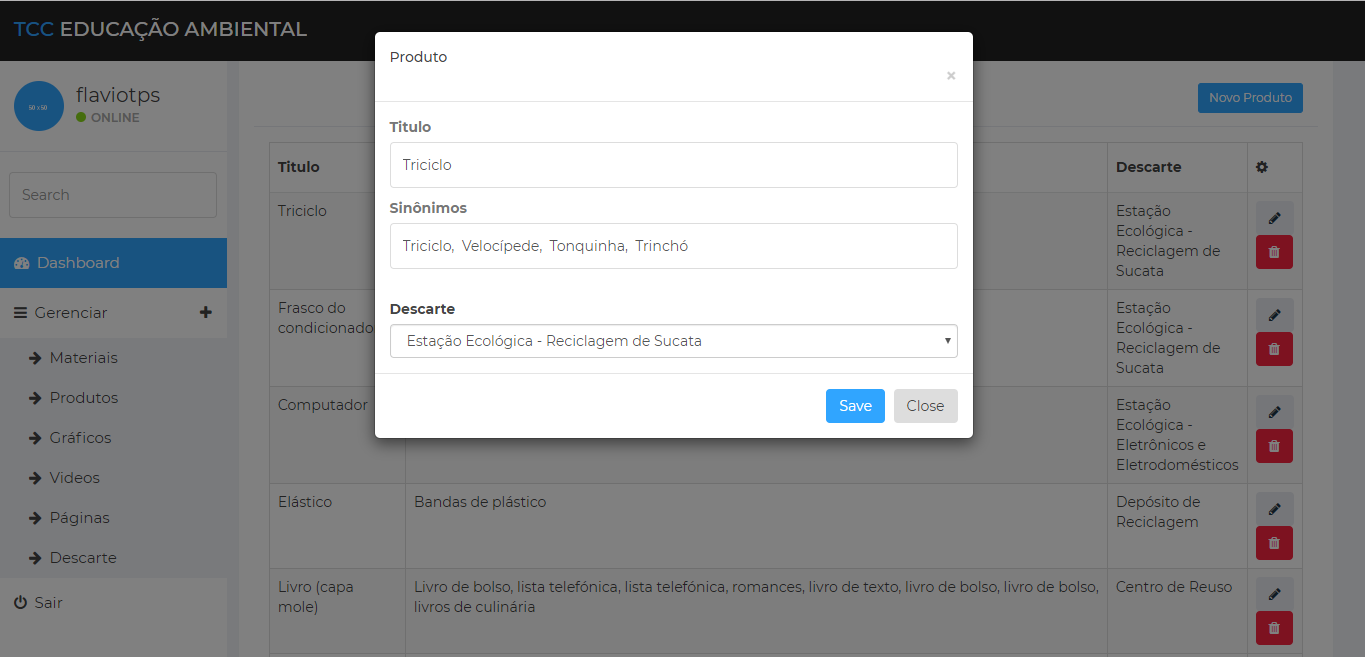
\includegraphics[scale=0.40]{media/tela_produto_site_2.png}
   \legend{Fonte: Autor}
     \label{fig:tela_produto_site_2}
\end{figure}

\newpage
\subsubsection{Tela de estatísticas}
A área de estatísticas permite adicionar gráficos do tipo \textit{PieChart} ou \textit{BarChart}. Os dados exibidos devem seguir uma sintaxe para que sejam exibidos corretamente.

\begin{figure}[h]
\centering
   \caption{Gráfico - Todos}
   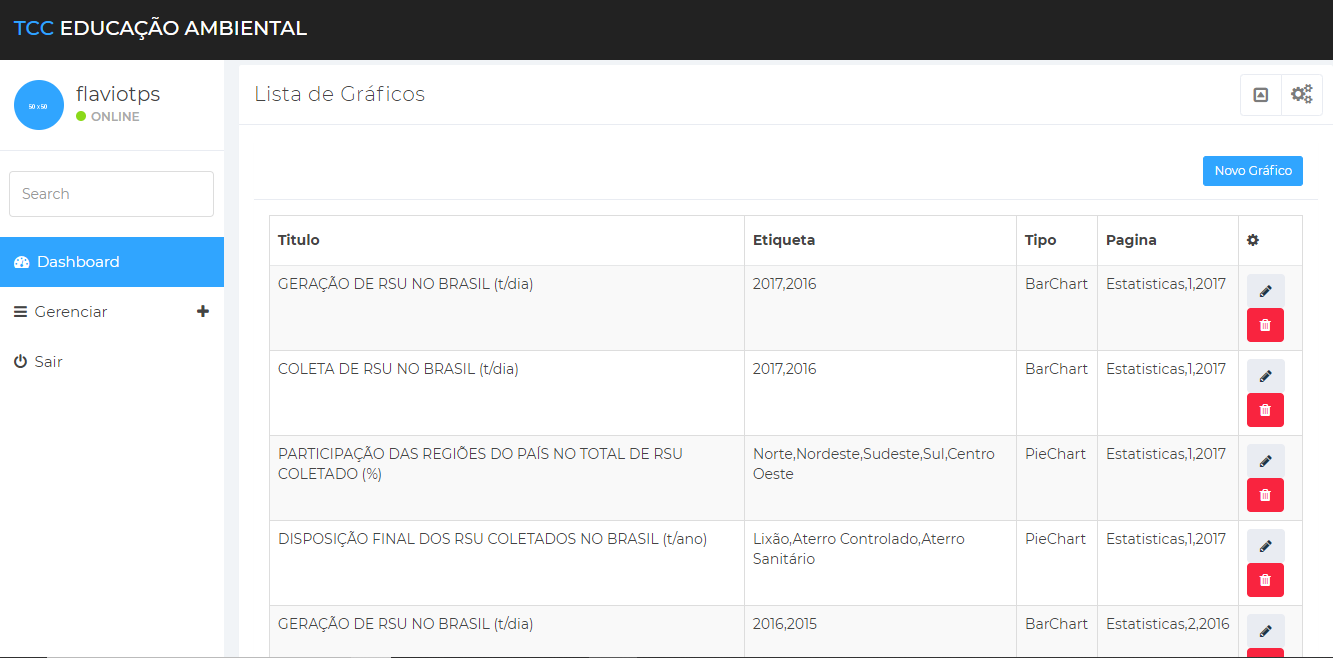
\includegraphics[scale=0.45]{media/tela_graficos_site_1.png}
   \legend{Fonte: Autor}
     \label{fig:tela_graficos_site_1}
\end{figure}

\begin{figure}[h]
\centering
   \caption{Gráfico - Edição}
   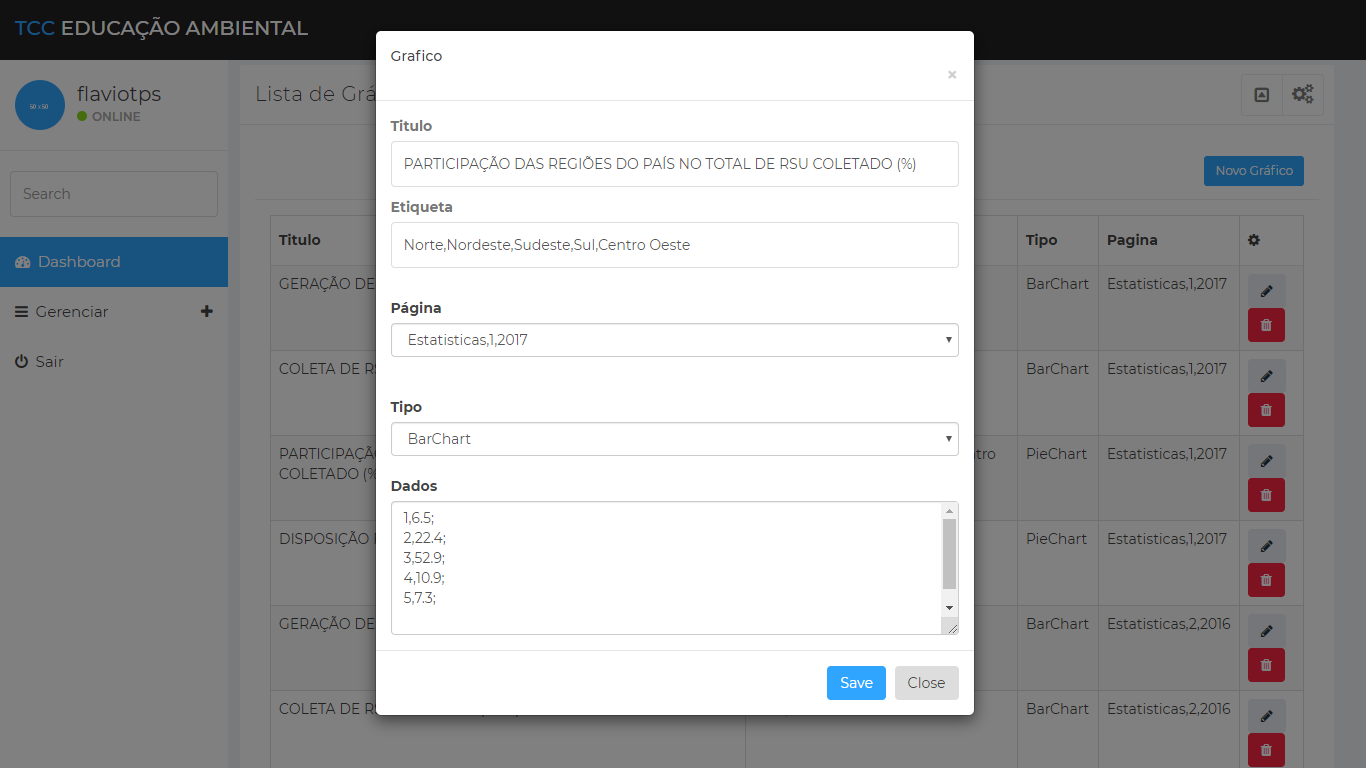
\includegraphics[scale=0.40]{media/tela_graficos_site_2.png}
   \legend{Fonte: Autor}
     \label{fig:tela_graficos_site_2}
\end{figure}

\newpage
\subsubsection{Tela de vídeos}
Nesta área é possível adicionar vídeos do \textit{youtube} relacionados ao tema através de um link. O vídeo fica disponível na sessão do vídeos do aplicativo.

\begin{figure}[h]
\centering
   \caption{Vídeo - Todos}
   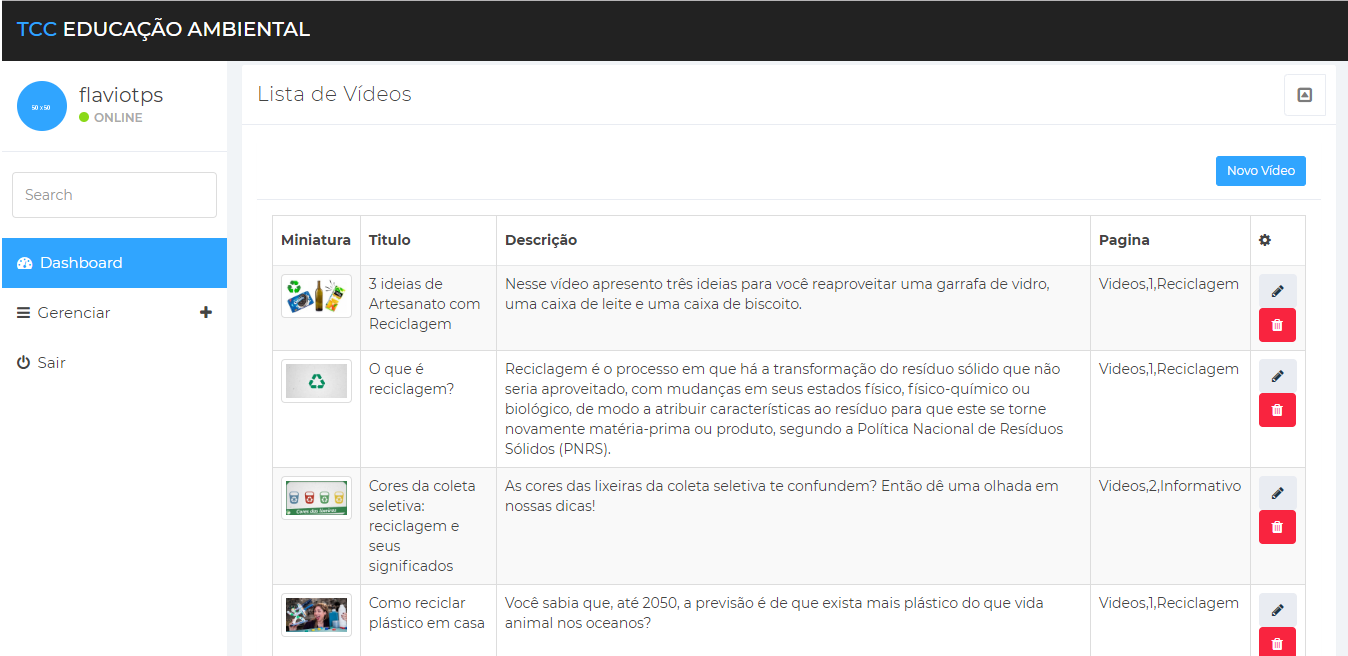
\includegraphics[scale=0.40]{media/tela_video_site_1.png}
   \legend{Fonte: Autor}
     \label{fig:tela_video_site_1}
\end{figure}

\begin{figure}[h]
\centering
   \caption{Vídeo - Edição}
   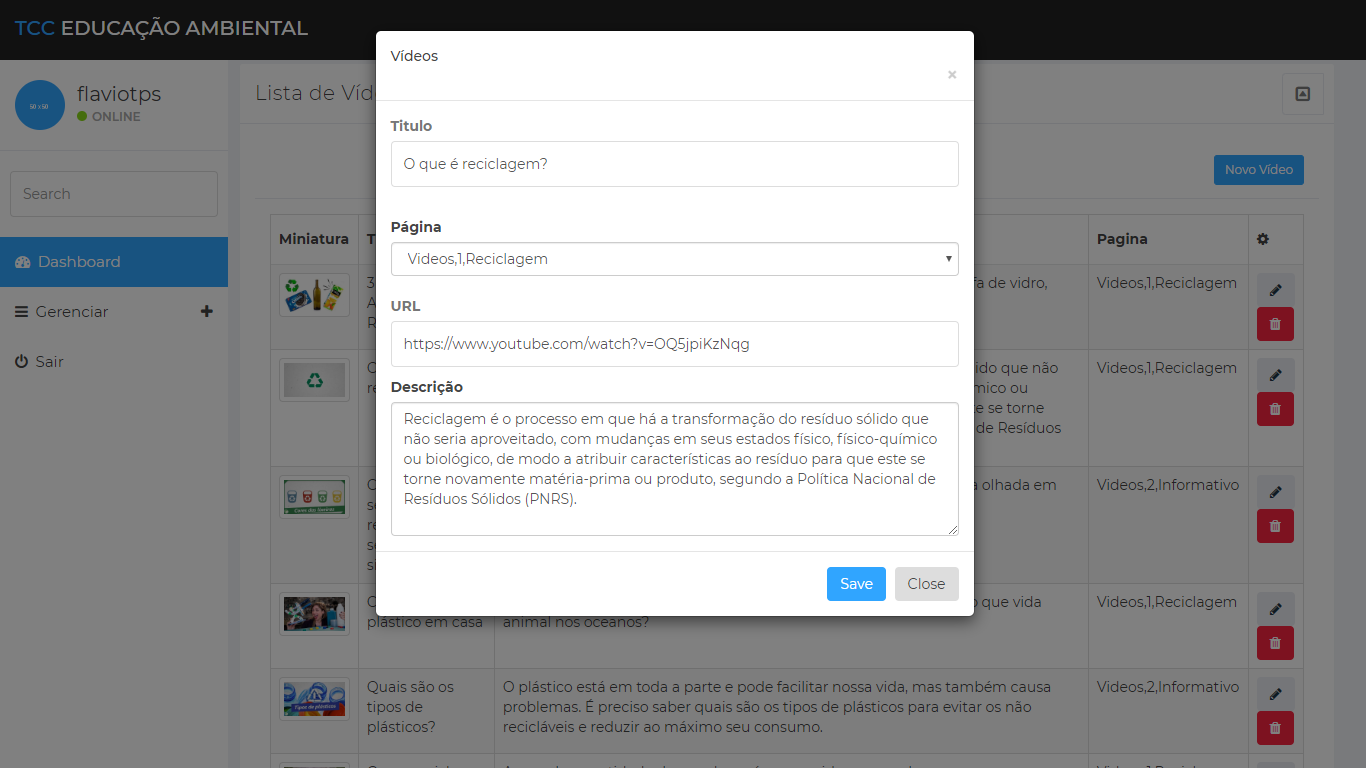
\includegraphics[scale=0.40]{media/tela_video_site_2.png}
   \legend{Fonte: Autor}
     \label{fig:tela_video_site_2}
\end{figure}

\newpage
\subsubsection{Tela de páginas}
Nesta área é possível criar paginas. As áreas de vídeos e gráficos fazem uso desse recurso para organização do conteúdo.

\begin{figure}[h]
\centering
   \caption{Página - Todas}
   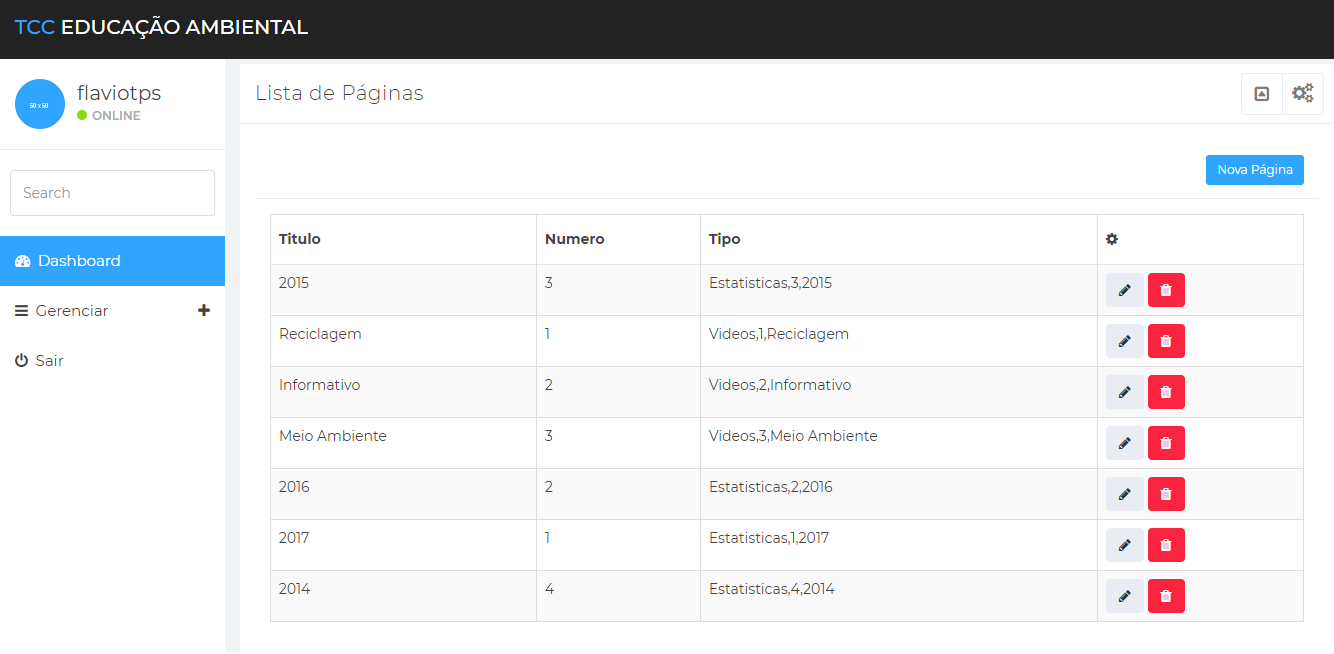
\includegraphics[scale=0.40]{media/tela_pagina_site_1.png}
   \legend{Fonte: Autor}
     \label{fig:tela_pagina_site_1}
\end{figure}

\begin{figure}[h]
\centering
   \caption{Página - Edição}
   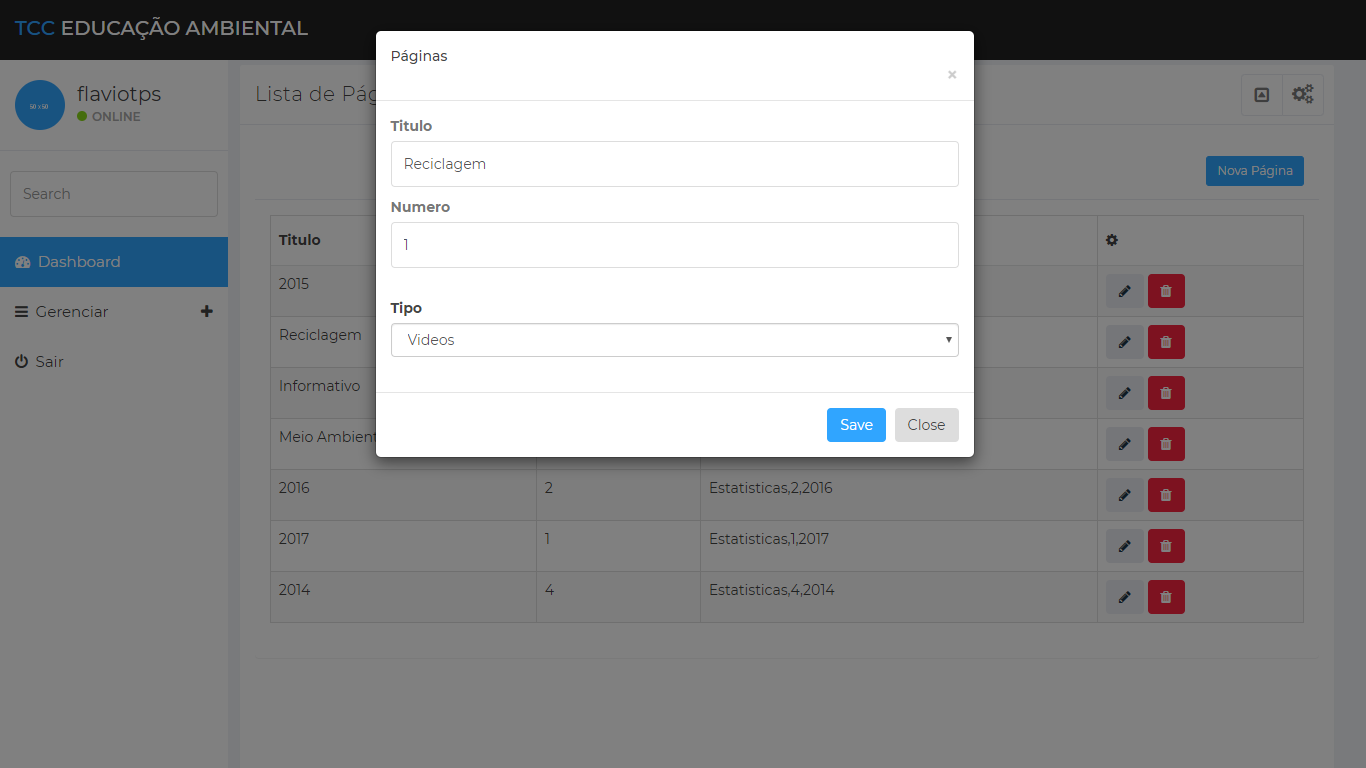
\includegraphics[scale=0.40]{media/tela_pagina_site_2.png}
   \legend{Fonte: Autor}
     \label{fig:tela_pagina_site_2}
\end{figure}
\newpage
\subsubsection{Tela de descartes}
Nesta área é possível criar formas de descarte para materiais. A área de produtos faz uso desse recurso.

\begin{figure}[h]
\centering
   \caption{Descarte - Todos}
   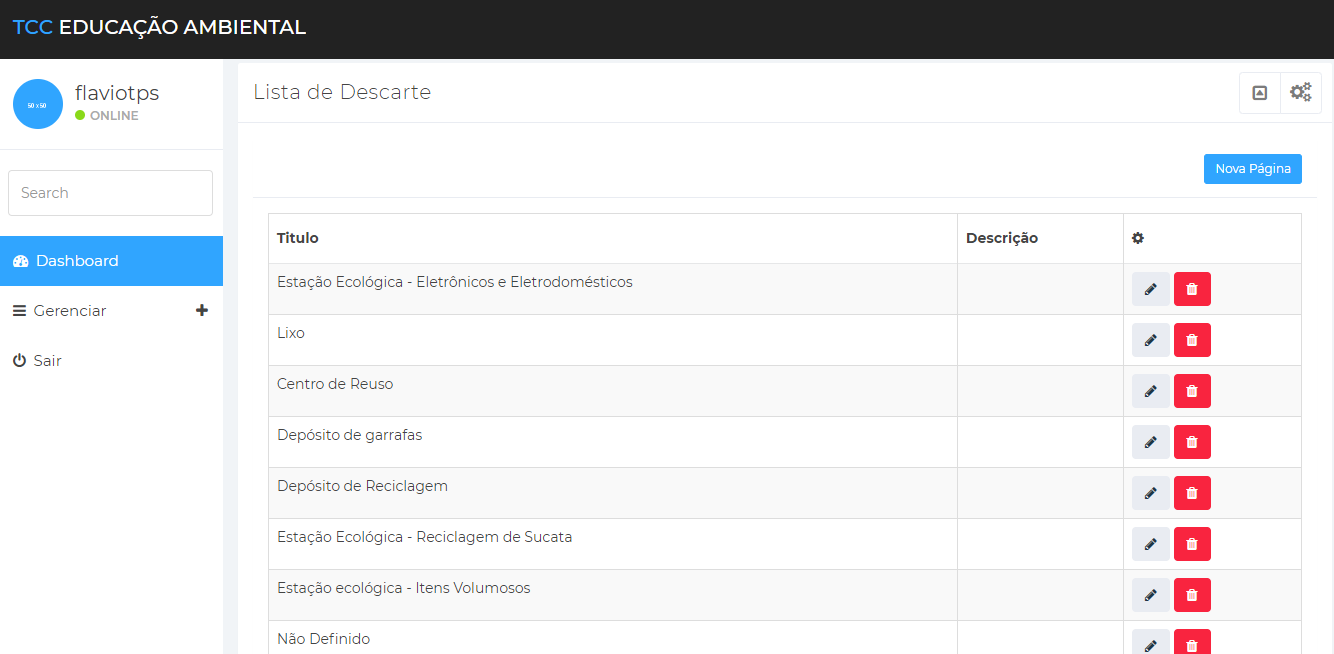
\includegraphics[scale=0.40]{media/tela_descarte_site_1.png}
   \legend{Fonte: Autor}
     \label{fig:tela_descarte_site_1}
\end{figure}

\begin{figure}[h]
\centering
   \caption{Descarte - Edição}
   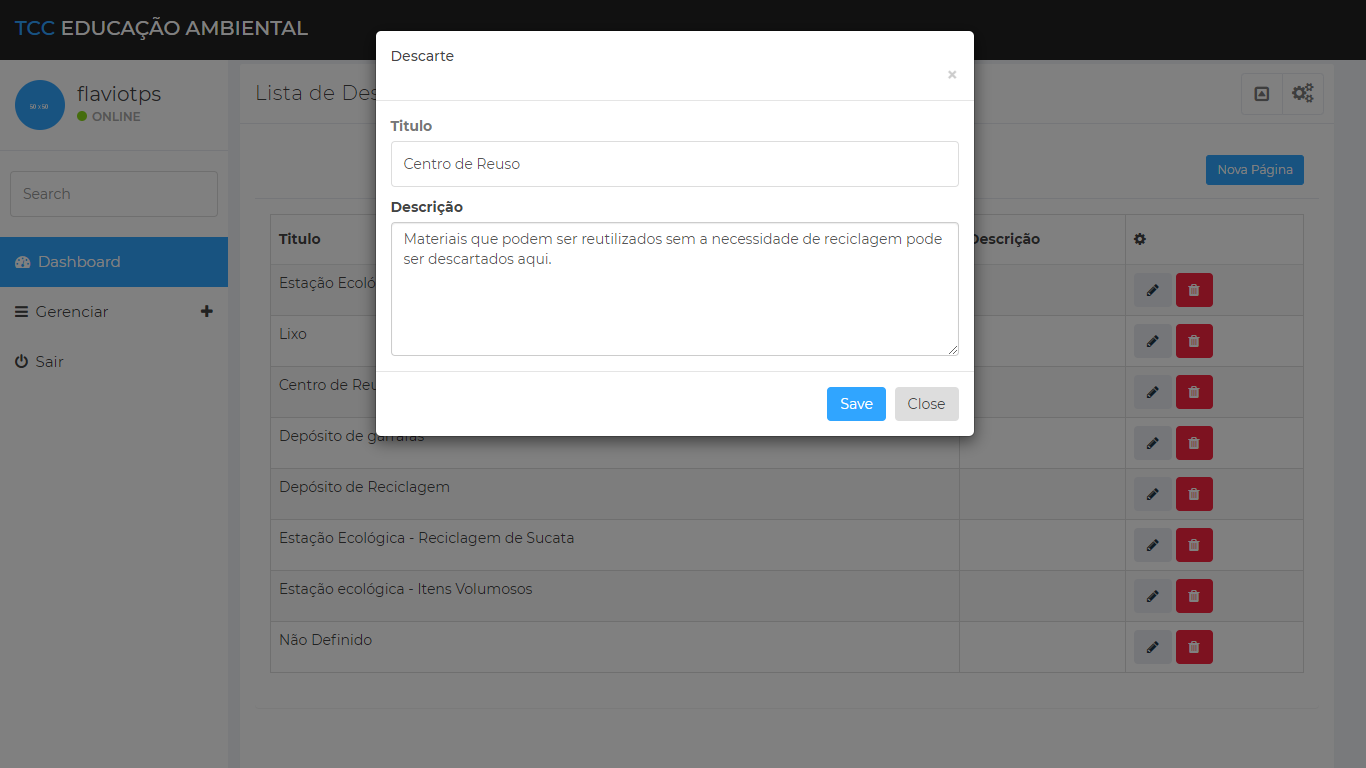
\includegraphics[scale=0.40]{media/tela_descarte_site_2.png}
   \legend{Fonte: Autor}
     \label{fig:tela_descarte_site_2}
\end{figure}
\subsection{Aplicativo}
Durante o processo de desenvolvimento foi utilizado arquivos \textit{XML} e arquivos \textit{Java}, os arquivos \textit{Java} são responsáveis por capturar os eventos do sistema e modelar as entidades, os arquivos \textit{XML} ficam responsáveis por desenhar a interface gráfica do aplicativo.
\subsubsection{Tela de carregamento}
A tela de carregamento também conhecida como \textit{splash screen} foi desenvolvida para carregar os dados que serão utilizados no aplicativo de forma paralela. Nesta etapa há uma verificação de conectividade, caso haja conexão com a internet o método \textit{getData} procura por atualizações, caso não haja conexão, os últimos dados carregados serão utilizados. O método \textit{getData} pode ser acessado pelo \textit{singleton} da classe \textit{DataRequestManager} que é recuperado a partir do método estático \textit{getInstance}. 

As animações de carregamento foram desenvolvidas utilizando a biblioteca \nameref{Lottie}.

    \begin{figure}[htb]    
 \centering
  \begin{minipage}{0.5\textwidth}
    \centering
    \caption{ Carregando}
    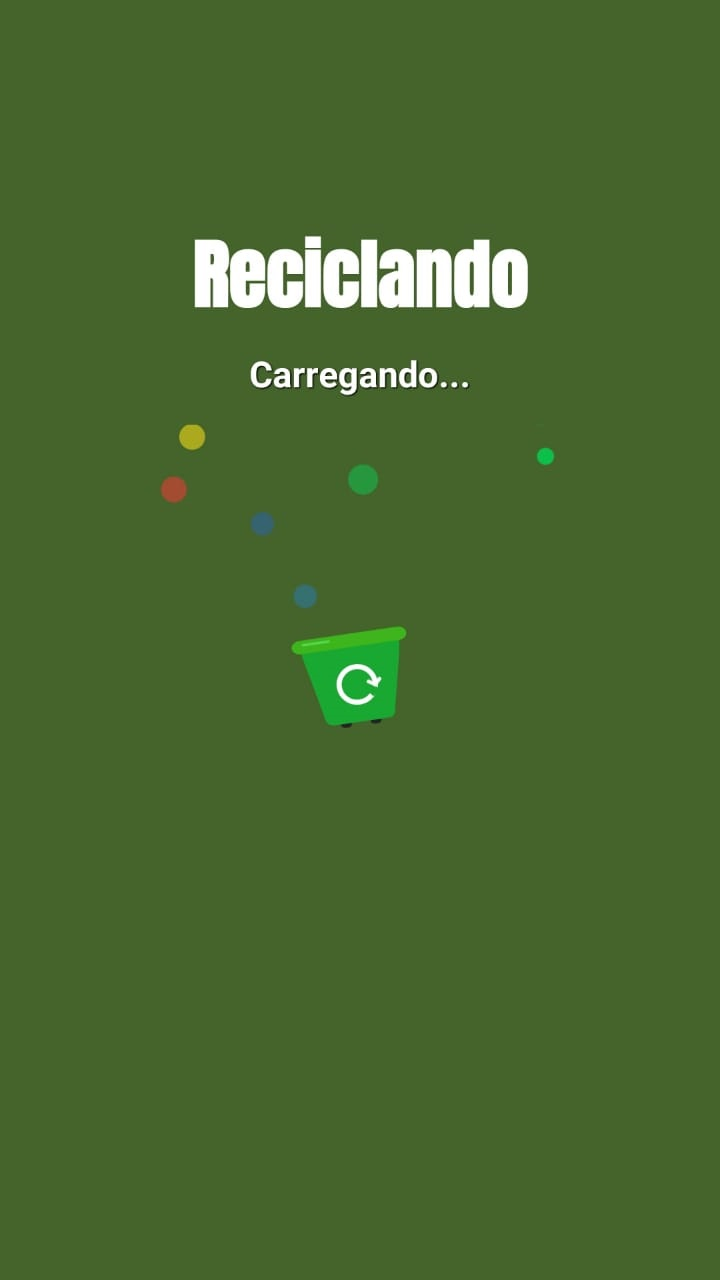
\includegraphics[scale=0.35]{media/tela_splash_1.jpg}
    \legend{Fonte: Autor}
     \label{fig:tela_splash_1_app}
  \end{minipage}
  \hfill
  \begin{minipage}{0.45\textwidth}
    \centering
    \caption{Carregado}
    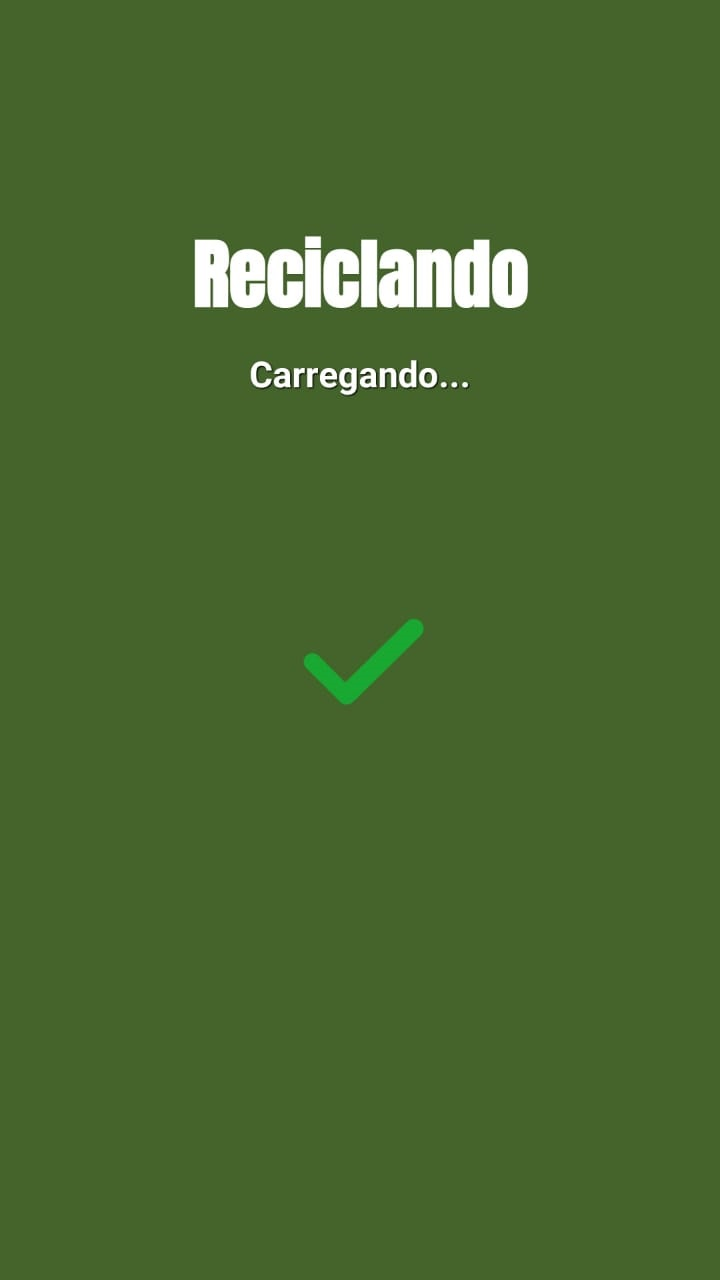
\includegraphics[scale=0.35]{media/tela_splash_2.jpg}
    \legend{Fonte: Autor}
     \label{fig:tela_splash_2_app}
  \end{minipage}
\end{figure}

\newpage
\begin{lstlisting}[numbers=none,basicstyle=\small,caption={Tela de carregamento - Java}, title={Tela de carregamento - Java}, label={ActivitySplash.java}]
public class ActivitySplash extends AppCompatActivity implements ICustomDialogClickListener {
    @Override
    protected void onCreate(Bundle savedInstanceState) {
        super.onCreate(savedInstanceState);
        Fabric.with(this, new Crashlytics());
        if ((getIntent().getFlags() & Intent.FLAG_ACTIVITY_BROUGHT_TO_FRONT) != 0) {
            finish();
            return;
        }
        getWindow().requestFeature(Window.FEATURE_NO_TITLE);
        getWindow().setFlags(WindowManager.LayoutParams.FLAG_FULLSCREEN,
        WindowManager.LayoutParams.FLAG_FULLSCREEN);
        setContentView(R.layout.activity_splash);
        getSupportActionBar().hide();
        switch (Helper.CheckConnection(this)) {
            case Constants.CONNECTION_OFFLINE:
                CustomConnectionDialog alert = new CustomConnectionDialog(this);
                alert.showDialog(this, getString(R.string.err_connection));
                break;
            default:
                DataRequestManager.getInstance(this).getData();
        }
    }
    @Override
    protected void onStop() {
        super.onStop();
        finish();
    }
    @Override
    public void OnOK() {
        DataRequestManager.getInstance(this).getData();
    }
}
\end{lstlisting}

\newpage
\begin{lstlisting}[numbers=none,basicstyle=\small,caption={Tela de carregamento - XML}, title={Tela de carregamento - XML}, label={ActivitySplash.java}]<?xml version="1.0" encoding="utf-8"?>
<androidx.constraintlayout.widget.ConstraintLayout xmlns:android="http://schemas.android.com/apk/res/android"
    xmlns:app="http://schemas.android.com/apk/res-auto"
    xmlns:tools="http://schemas.android.com/tools"
    android:orientation="vertical"
    android:background="@color/colorPrimaryDark"
    android:layout_width="match_parent"
    android:layout_height="match_parent">
    
    <TextView
        android:id="@+id/SplashAppTitle"
        android:layout_width="0dp"
        android:layout_height="wrap_content"
        android:layout_marginStart="8dp"
        android:layout_marginTop="100dp"
        android:layout_marginEnd="8dp"
        android:fontFamily="@font/anton"
        android:text="Reciclando"
        android:textAlignment="center"
        android:textColor="@color/white"
        android:textSize="38sp"
        android:textStyle="bold"
        app:layout_constraintEnd_toEndOf="parent"
        app:layout_constraintStart_toStartOf="parent"
        app:layout_constraintTop_toTopOf="parent"
        tools:text="Reciclando" />

    <TextView
        android:id="@+id/splash_status"
        android:layout_width="wrap_content"
        android:layout_height="wrap_content"
        android:layout_marginTop="8dp"
        android:shadowColor="#000000"
        android:shadowDx="1.5"
        android:shadowDy="1.3"
        android:shadowRadius="1.6"
        android:text="Carregando..."
        android:textColor="@color/white"
        android:textSize="18sp"
        android:textStyle="bold"
        app:layout_constraintEnd_toEndOf="parent"
        app:layout_constraintStart_toStartOf="parent"
        app:layout_constraintTop_toBottomOf="@+id/SplashAppTitle" />
        
    <com.airbnb.lottie.LottieAnimationView
        android:id="@+id/animation_view"
        android:scaleType="centerCrop"
        app:lottie_rawRes="@raw/loading_trash"
        android:layout_width="250dp"
        android:layout_height="250dp"
        android:layout_marginTop="32dp"
        android:layout_marginBottom="196dp"
        android:indeterminate="true"
        android:indeterminateTint="@color/white"
        android:indeterminateTintMode="src_atop"
        android:visibility="visible"
        app:layout_constraintBottom_toBottomOf="parent"
        app:layout_constraintEnd_toEndOf="@+id/splash_status"
        app:layout_constraintStart_toStartOf="@+id/splash_status"
        app:layout_constraintTop_toBottomOf="@+id/splash_status" />

</androidx.constraintlayout.widget.ConstraintLayout>
\end{lstlisting}
\subsubsection{Tela principal}
\subsubsection{Tela de materiais}
\subsubsection{Tela de produtos}
\subsubsection{Tela de estatísticas}
\subsubsection{Tela de vídeos}
\subsubsection{Tela de locais}
\end{chapter}

% ----------------------------------------------------------
\chapter{Conclusão}

% ----------------------------------------------------------
\chapter{Trabalhos futuros}



% ----------------------------------------------------------
% ELEMENTOS PÓS-TEXTUAIS
% ----------------------------------------------------------
\postextual
% ----------------------------------------------------------

% ----------------------------------------------------------
% Referências bibliográficas
% ----------------------------------------------------------

\bibliographystyle{alpha}
\bibliography{bibliography.bib}




% ----------------------------------------------------------
% Glossário
% ----------------------------------------------------------
%
% Consulte o manual da classe abntex2 para orientações sobre o glossário.
%
%\glossary

% ----------------------------------------------------------
% Apêndices
% ----------------------------------------------------------





%---------------------------------------------------------------------
% INDICE REMISSIVO
%---------------------------------------------------------------------
\phantompart
\printindex
%---------------------------------------------------------------------

\end{document}
